\documentclass[spanish,unknownkeysallowed,10pt]{beamer}
%% \usetheme{Warsaw}
%% \usetheme{Madrid}

\usepackage[spanish]{babel}
\usetheme[beetle]{Boadilla}


 \useoutertheme{miniframes}
%% \useinnertheme{rounded}
%% \usecolortheme{}
\usepackage[utf8]{inputenc}
\usepackage{tikz}
\usepackage{wrapfig}
\usepackage{algorithmic, algorithm}
%% \usepackage{authblk}


%% \setbeameroption{show notes}


\usepackage{graphicx} 
%\usepackage{multimedia} 
\usepackage{xmpmulti}
\usepackage{animate}


%\usepackage{algorithmic}
%\usepackage{algorithm}
\newcommand{\formulasize}{\tiny}

\definecolor{rojo}{rgb}{0.7,0.1,0.1}
\definecolor{azul}{rgb}{0.1,0.1,0.7}
\definecolor{verde}{rgb}{0.1,0.4,0.1}

\newcommand{\rojo}[1]{\textcolor{rojo}{#1}}
\newcommand{\azul}[1]{\textcolor{azul}{#1}}
\newcommand{\verde}[1]{\textcolor{verde}{#1}}

%% \setcounter{secnumdepth}{5}

\newcommand{\Rojo}[1]{\textbf{\rojo{#1}}}
\newcommand{\Azul}[1]{\textbf{\azul{#1}}}
\newcommand{\Verde}[1]{\textbf{\verde{#1}}}

%%% Unified concepts commands

\newcommand{\opencl}{\emph{OpenCL}}

\newcommand{\pipeline}{\emph{pipeline}}
\newcommand{\Pipeline}{\emph{Pipeline}}

\newcommand{\wi}{\emph{work item}}
\newcommand{\wis}{\emph{work items}}
\newcommand{\wg}{\emph{work group}}
\newcommand{\wgs}{\emph{work groups}}

\newcommand{\Wi}{\emph{Work item}}
\newcommand{\Wis}{\emph{Work items}}
\newcommand{\Wg}{\emph{Work group}}
\newcommand{\Wgs}{\emph{Work groups}}

\newcommand{\bbox}{BBox}
\newcommand{\bboxes}{BBoxes}
\newcommand{\bvh}{BVH}
\newcommand{\bvhs}{BVHs}

\newcommand {\raytracer}{\emph{ray tracer}}
\newcommand {\raytracers}{\emph{ray tracers}}
\newcommand {\raytracing}{\emph{ray tracing}}
\newcommand {\Raytracer}{\emph{Ray tracer}}
\newcommand {\Raytracers}{\emph{Ray tracers}}
\newcommand {\Raytracing}{\emph{Ray tracing}}

%%% Style fix so institue doesnt appear on brackets (props to Claudio Fiandrino)
\setbeamertemplate{footline}{
  \leavevmode%
  \hbox{%
  \begin{beamercolorbox}[wd=.333333\paperwidth,ht=2.25ex,dp=1ex,center]{author in head/foot}%
    \usebeamerfont{author in head/foot}\insertshortauthor
  \end{beamercolorbox}%
  \begin{beamercolorbox}[wd=.333333\paperwidth,ht=2.25ex,dp=1ex,center]{title in head/foot}%
    \usebeamerfont{title in head/foot}\insertshorttitle
  \end{beamercolorbox}%
  \begin{beamercolorbox}[wd=.333333\paperwidth,ht=2.25ex,dp=1ex,right]{date in head/foot}%
    \usebeamerfont{date in head/foot}\insertshortdate{}\hspace*{2em}
    \insertframenumber{} / \inserttotalframenumber\hspace*{2ex} 
  \end{beamercolorbox}}%
  \vskip0pt%
}

\begin{document}
\title
    [Modelado Foto-Realístico de Materiales]{Modelado y Simulación Foto-Realística de Materiales}

\author[Lic. Rodrigo Baravalle]{Lic. Rodrigo Baravalle}
 
\institute[UNR]{
    FCEIA, Universidad Nacional de Rosario. CIFASIS-CONICET.
}

\date{Tesis Doctoral, 28 de Marzo de 2016}

\begin{frame}
\begin{figure}
{
\includegraphics[width=0.08\textwidth]{../figures/logounr}}
\end{figure}
\vspace{-1cm}
  \titlepage
\centering
\vspace{-.4cm}
\begin{tiny}
Director: Dr. Claudio Delrieux, UNS

Co-Director: Dr. Juan Carlos Gómez, UNR

\ \\

\it{Miembros del jurado:}

Dr. Néstor Calvo (UNL)

Dr. Marcelo Vénere (UNICEN)

Dr. Gustavo Galizzi (UNR)

\end{tiny}

\end{frame}
%%%%%%%%%%%%%%%%%%%%%%%%%%%

\section{Introducción}

\begin{frame}
\begin{block}{}
\begin{center}
\vspace{1cm}
\huge{Introducción}
\vspace{1cm}
\end{center}
\end{block}
\end{frame}


\subsection{Modelado y Simulación Foto-Realística}
\begin{frame}{}

\centerline{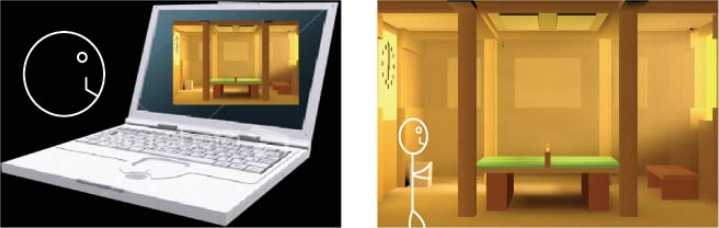
\includegraphics[scale = 0.2]{../figures/fotorealismo}}

\textbf{Foto-realismo}: síntesis de imágenes en una \textbf{computadora}, que produzcan el \textbf{mismo efecto}, en la \textbf{percepción}, que una fotografía

\vspace{0.2cm}

Avances notables (\textbf{realismo}, \textbf{velocidad})

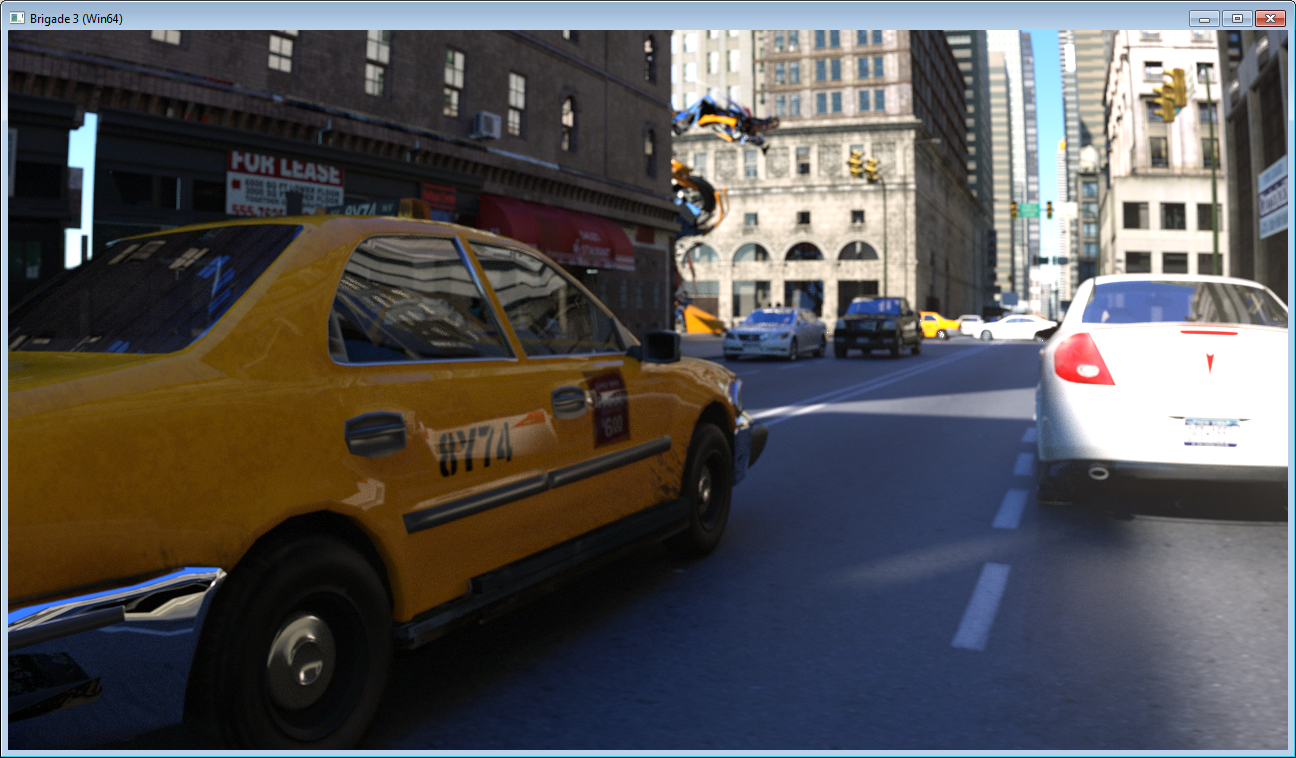
\includegraphics[scale = 0.15]{../figures/brigade3}
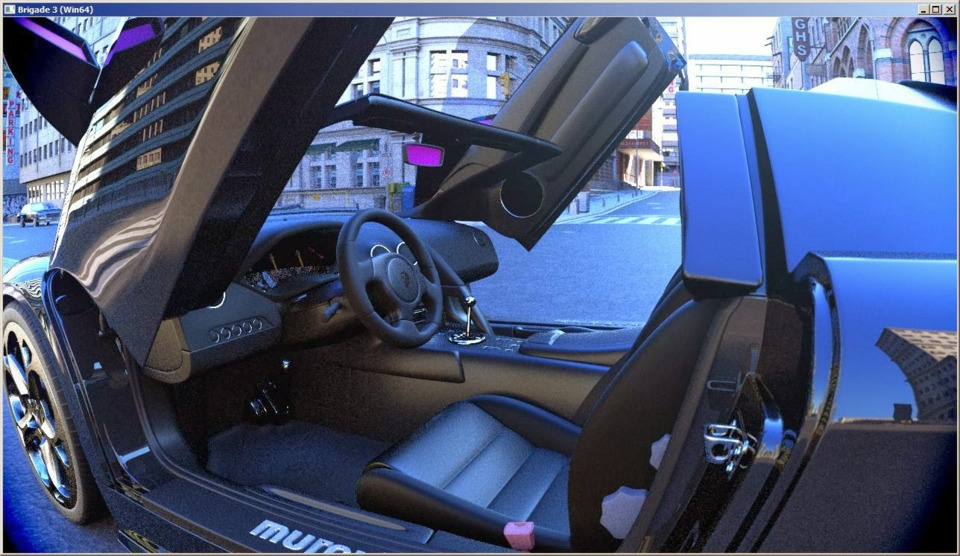
\includegraphics[scale = 0.15]{../figures/brigade3_2}

Brigade 3 Renderer: tiempo real!

\end{frame}


\begin{frame}{}

\textbf{Síntesis de imágenes $\leftrightarrow$ Renderización}:

Computar \textbf{radiancia entrante}:  \textbf{cámara}  $\leftarrow$ \textbf{escena}

\vspace{0.2cm}

\begin{block}{Debe modelarse}
\begin{itemize}
\item \textbf{Luz Visible} (líneas rectas o \textbf{Rayos})
\item Interacción Luz $\leftrightarrow$ \textbf{cada} material
\end{itemize}
\end{block}

\vspace{0.2cm}

Modelar \textbf{apariencia} de un material:

\textbf{micro-geometría}, \textbf{macro-geometría}, \textbf{color}, \textbf{forma}, temperatura, etc.

\vspace{0.2cm}

Estudio de la \textbf{apariencia} de un material $\rightarrow$ Modelo Numérico

\centerline{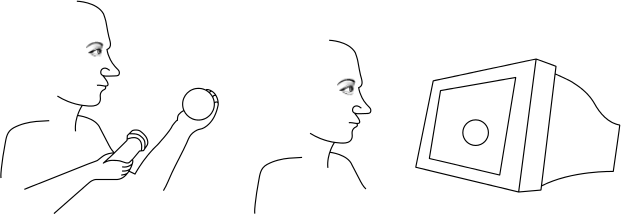
\includegraphics[scale = 0.25]{../figures/apariencia}}

\end{frame}

\subsection{Modelado de Materiales}

\begin{frame}{}

Modelado de \textbf{Geometría} de Materiales

\begin{block}{}
Técnicas algorítmicas. Sistemas-L (\textbf{Comparación subjetiva}: sintético $\leftrightarrow$ real)

\center

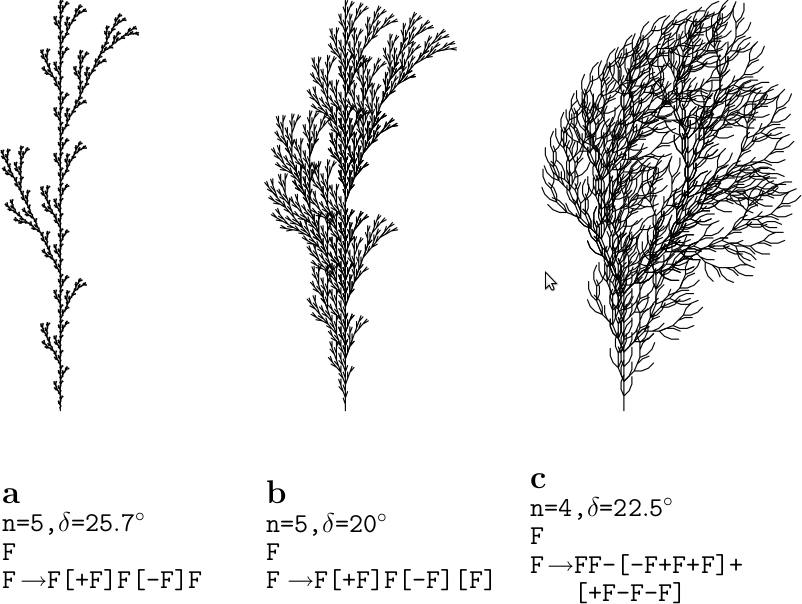
\includegraphics[width=3.7cm]{../figures/sistemalcorchete}
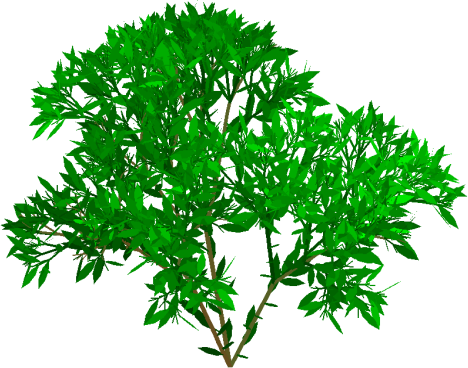
\includegraphics[width=3.54cm]{../figures/3dlsystem}

\end{block}
\begin{block}{}

Ecuaciones de \textbf{comportamiento}, \textbf{crecimiento}. Navier-Stokes (fluídos)
\center
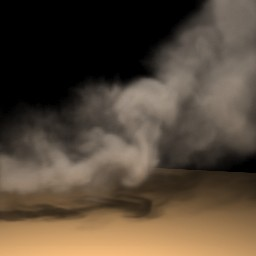
\includegraphics[width=2.385cm]{../figures/smoke}
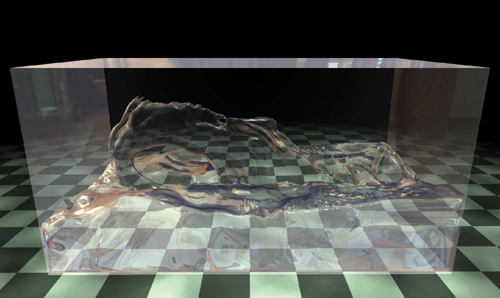
\includegraphics[width=4cm]{../figures/water}
\end{block}

\end{frame}


\begin{frame}{}

\begin{block}{Materiales con mayor aparición en la literatura}

Agua, Piel humana, Metales, Plásticos, etc. 

\textbf{Facilidad} del diseño, ubicuidad

\end{block}

\begin{block}{Materiales con menor aparición en la literatura}
Cocidos, porosos y comestibles

\textbf{Geometría compleja y visible}, \textbf{fácil detección} de modelos inadecuados, \textbf{costo computacional}


{\it Alain Fournier: `computer graphics has still not been
able to convincingly render a slice of bread' (2001)}
\end{block}


\begin{block}{}
En esta tesis haremos hincapié en materiales \textbf{porosos} para Computación Gráfica (CG).

Obtener \textbf{geometría} configurable, intuitiva y creíble de estos materiales para \textbf{renderización foto-realista} en tiempo interactivo/real.

\end{block}

\end{frame}

\begin{frame}{Esquema de la Charla}

\begin{block}{Esquema de la Charla}
\begin{itemize}
\item Modelado \textbf{procedimental} de materiales porosos
\item Modelado \textbf{procedimental} del proceso de formación del pan
\item Renderización de materiales porosos
\item Conclusiones, Trabajos a Futuro
\end{itemize}
\end{block}

\end{frame}

\section[Mod. de Materiales Porosos]{Modelado Procedimental de Materiales Porosos}

\begin{frame}
\begin{block}{}
\begin{center}
\vspace{1cm}
\huge{Modelado Procedimental de Materiales Porosos}
\vspace{1cm}
\end{center}
\end{block}
\end{frame}

\subsection{Modelado de Materiales Porosos}

\begin{frame}{Modelado de Geometrías Porosas (CG) - Trabajo Previo}

\textbf{Volúmenes}: Ratatouille Película (Reporte técnico)

Ruido Voronoi, Perlin, Worley. $+$ consideraciones ad-hoc (el usuario debe ser \textbf{experto})

\centerline{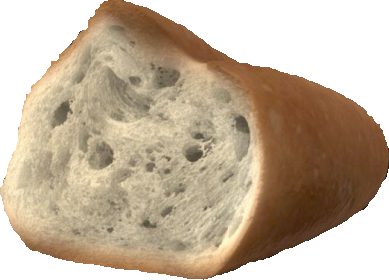
\includegraphics[scale = 0.2]{../figures/ratatouille}}

\textbf{Superficies}: {\it Tong et al (2005)}

Capturas (cámaras y lásers) $\rightarrow$ radiancia.

Proceso de captura muy complejo, limitado a una geometría. Tiempos de cómputo?, cortes

\centerline{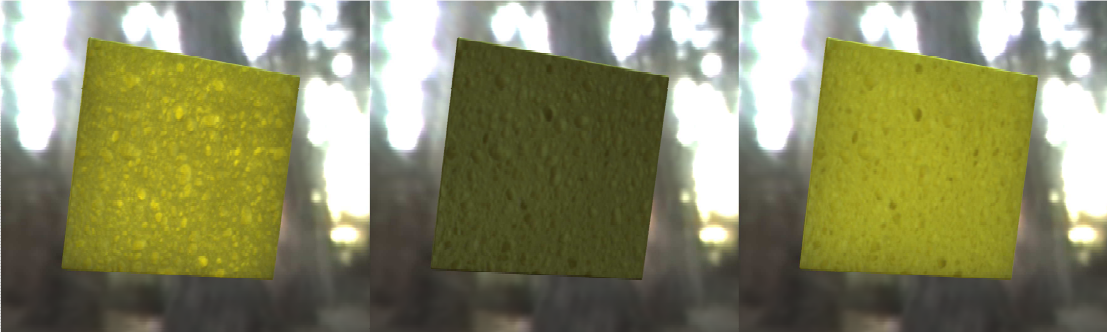
\includegraphics[scale = 0.2]{../figures/esponja}}

\end{frame}


\begin{frame}{Propuesta}
Presentamos un modelo \textbf{procedimental}, semi-automático de generación de geometrías porosas
\begin{itemize}
\item \textbf{Sistemas de Partículas} que crecen, evitándose
\item \textbf{Sistemas dinámicos} como medio de crecimiento
\end{itemize}

\vspace{0.4cm}

\textbf{Sistemas de partículas}

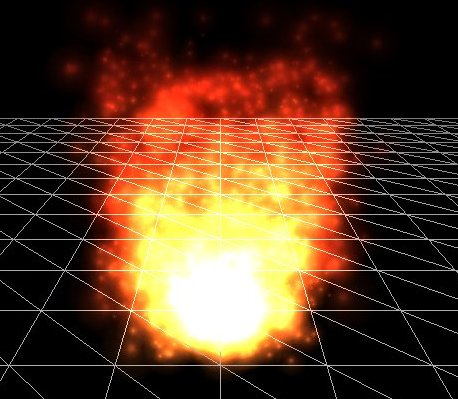
\includegraphics[scale = 0.216]{../figures/fire}
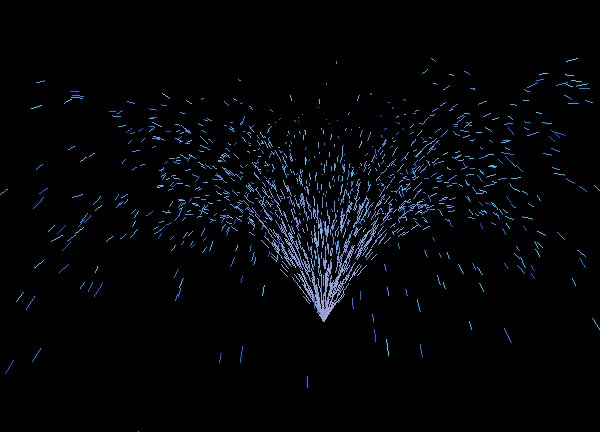
\includegraphics[scale = 0.2]{../figures/fireworks}
\end{frame}

\begin{frame}
\textbf{Propuesta}
\begin{itemize}
\item $P$: partículas (conjunto)
\item $L$, $L^{2}$: texturas 3D
\end{itemize}

\begin{itemize}
\item  $p_{i} = \{O_{i}, C_{i}\}$
\end{itemize}

\begin{itemize}
\item $O_{i}$: posiciones ocupadas en $L$, $C_{i}$: {\em contorno} en $L$.
\end{itemize}

\textbf{Inicio}: cada partícula ocupa una posición aleatoria. Iterar sobre cada partícula

Posición $\rightarrow$ Chequear que los \textbf{vecinos} de la posición estén libres

\centerline{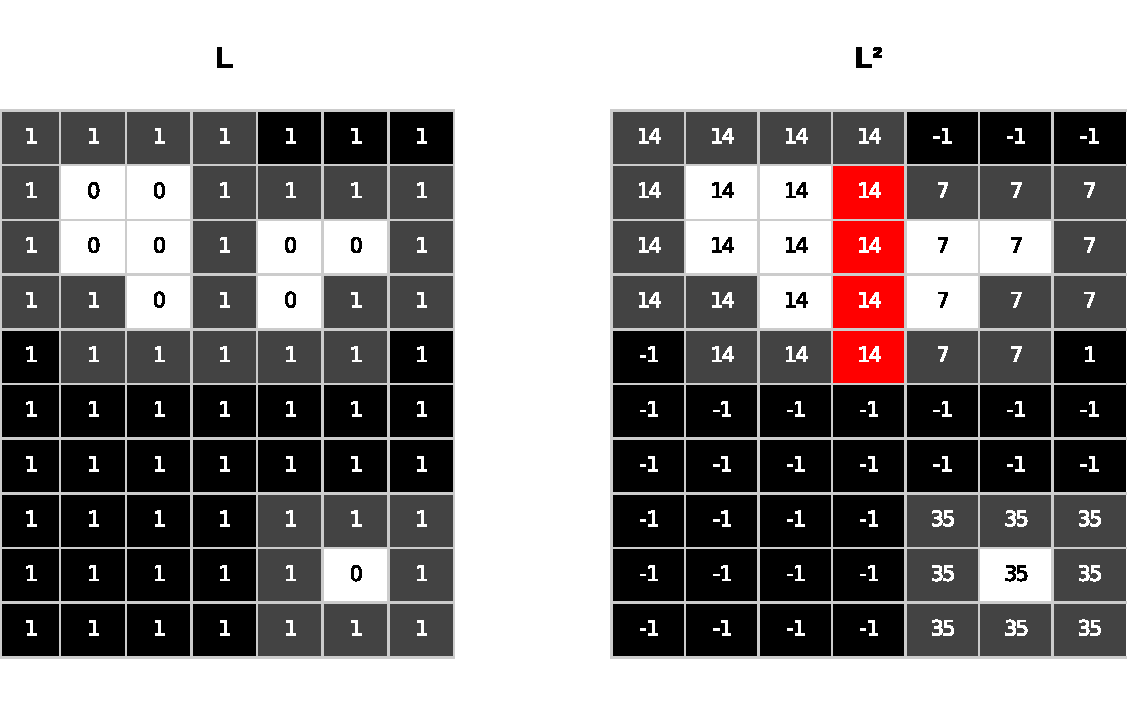
\includegraphics[scale = 0.35]{../figures/sistemaparticulas}}

\end{frame}

\begin{frame}{Ejemplo: crecimiento}
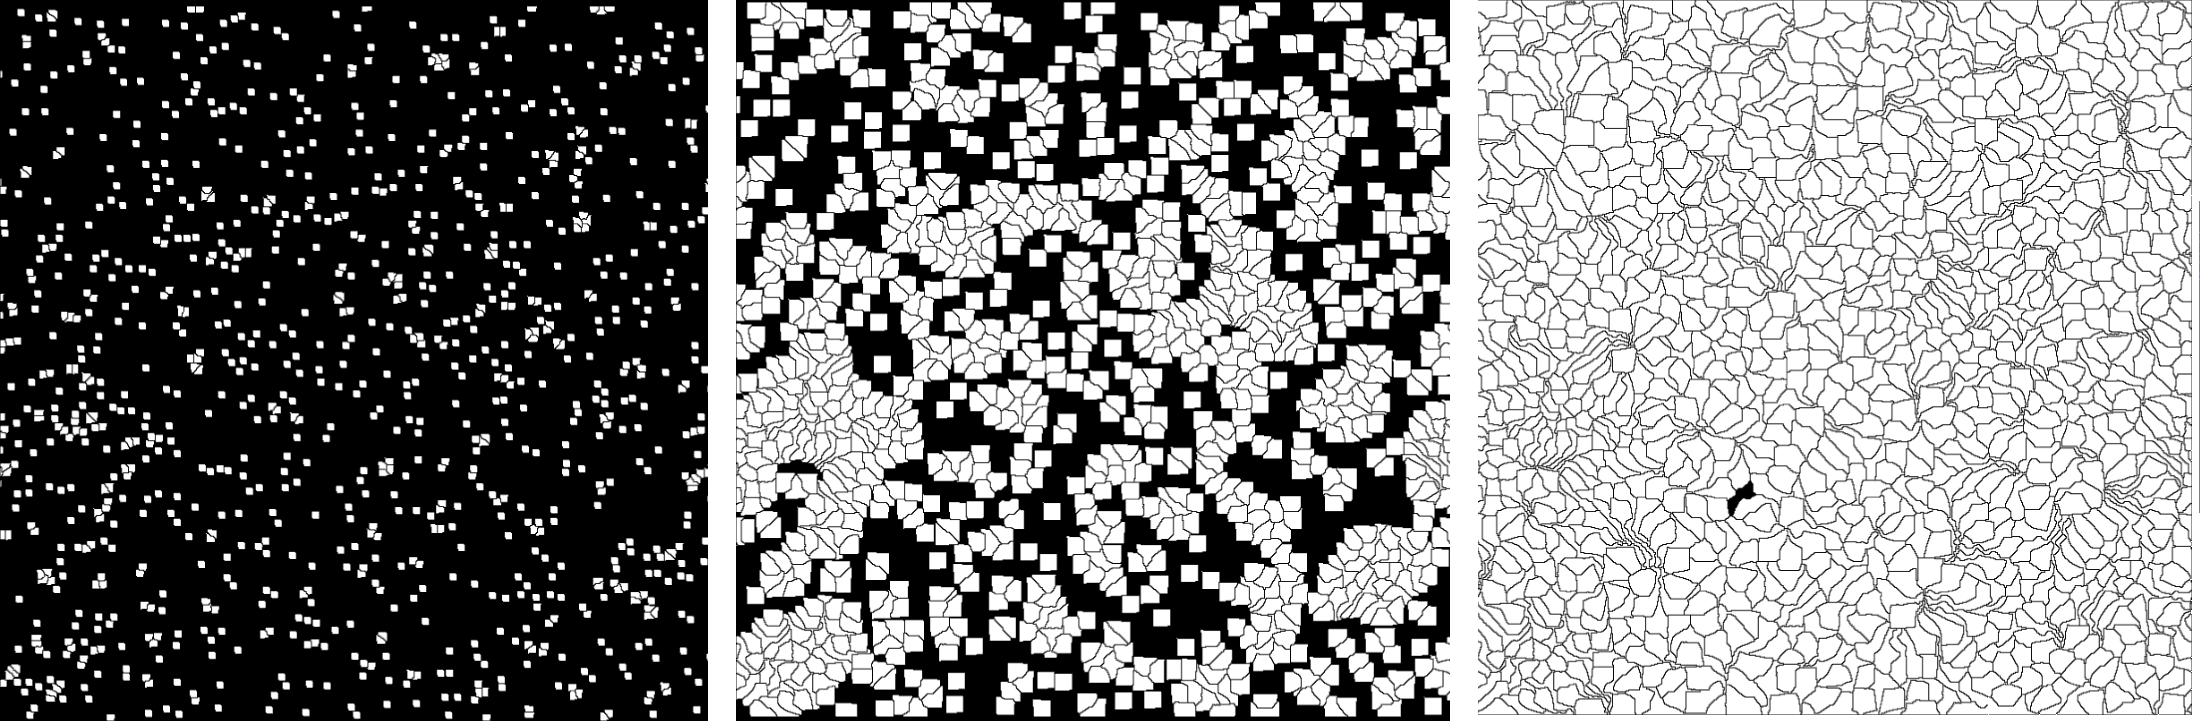
\includegraphics[scale = 0.12]{../figures/modeladocrec}

\vspace{0.1cm}

Sistema Dinámico (SD) $\rightarrow$ campo vectorial (discreto) $\rightarrow$ dirección

\centerline{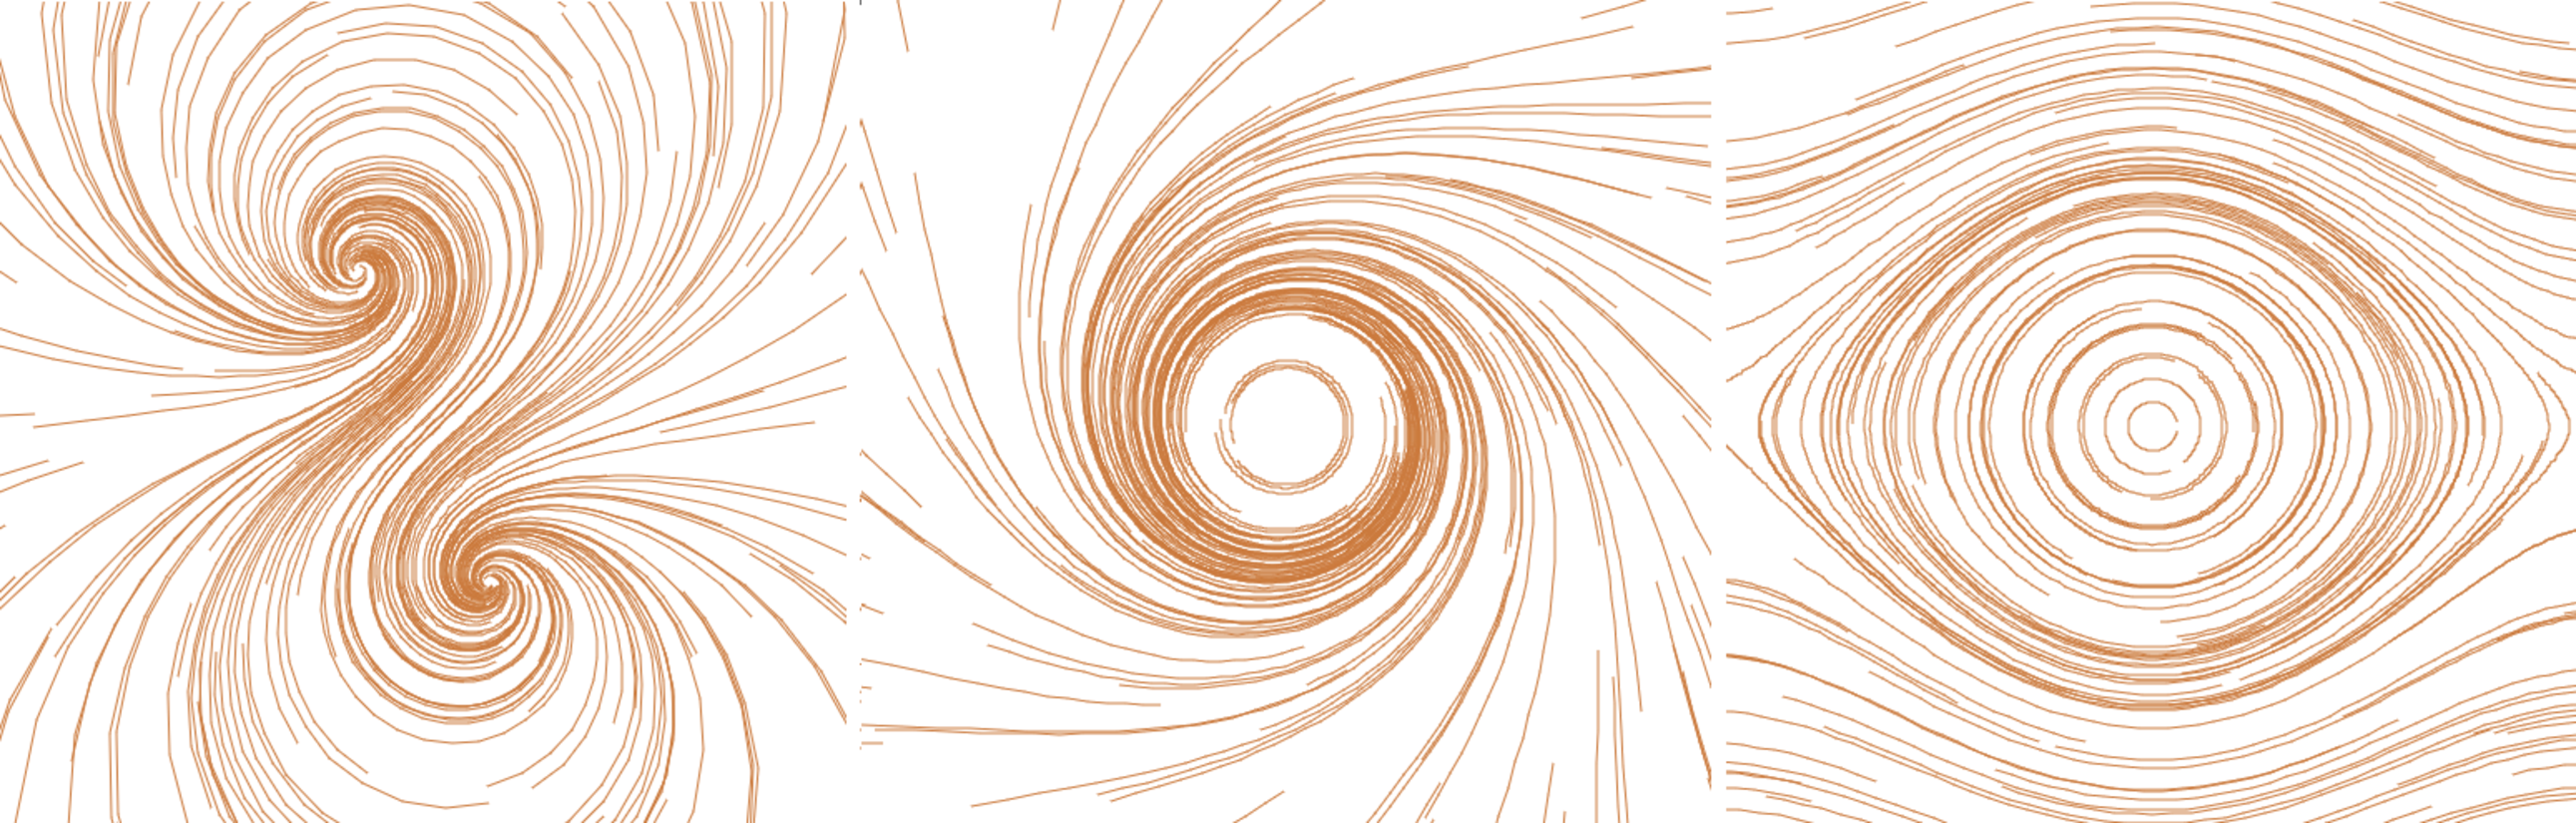
\includegraphics[width=8cm]{../figures/Fig2}}


\end{frame}

\begin{frame}{Sistemas de partículas + Sistemas Dinámicos}

\centering
Aleatoriedad = 0.3, 0.2, y 0.1

\vspace{0.1cm}
  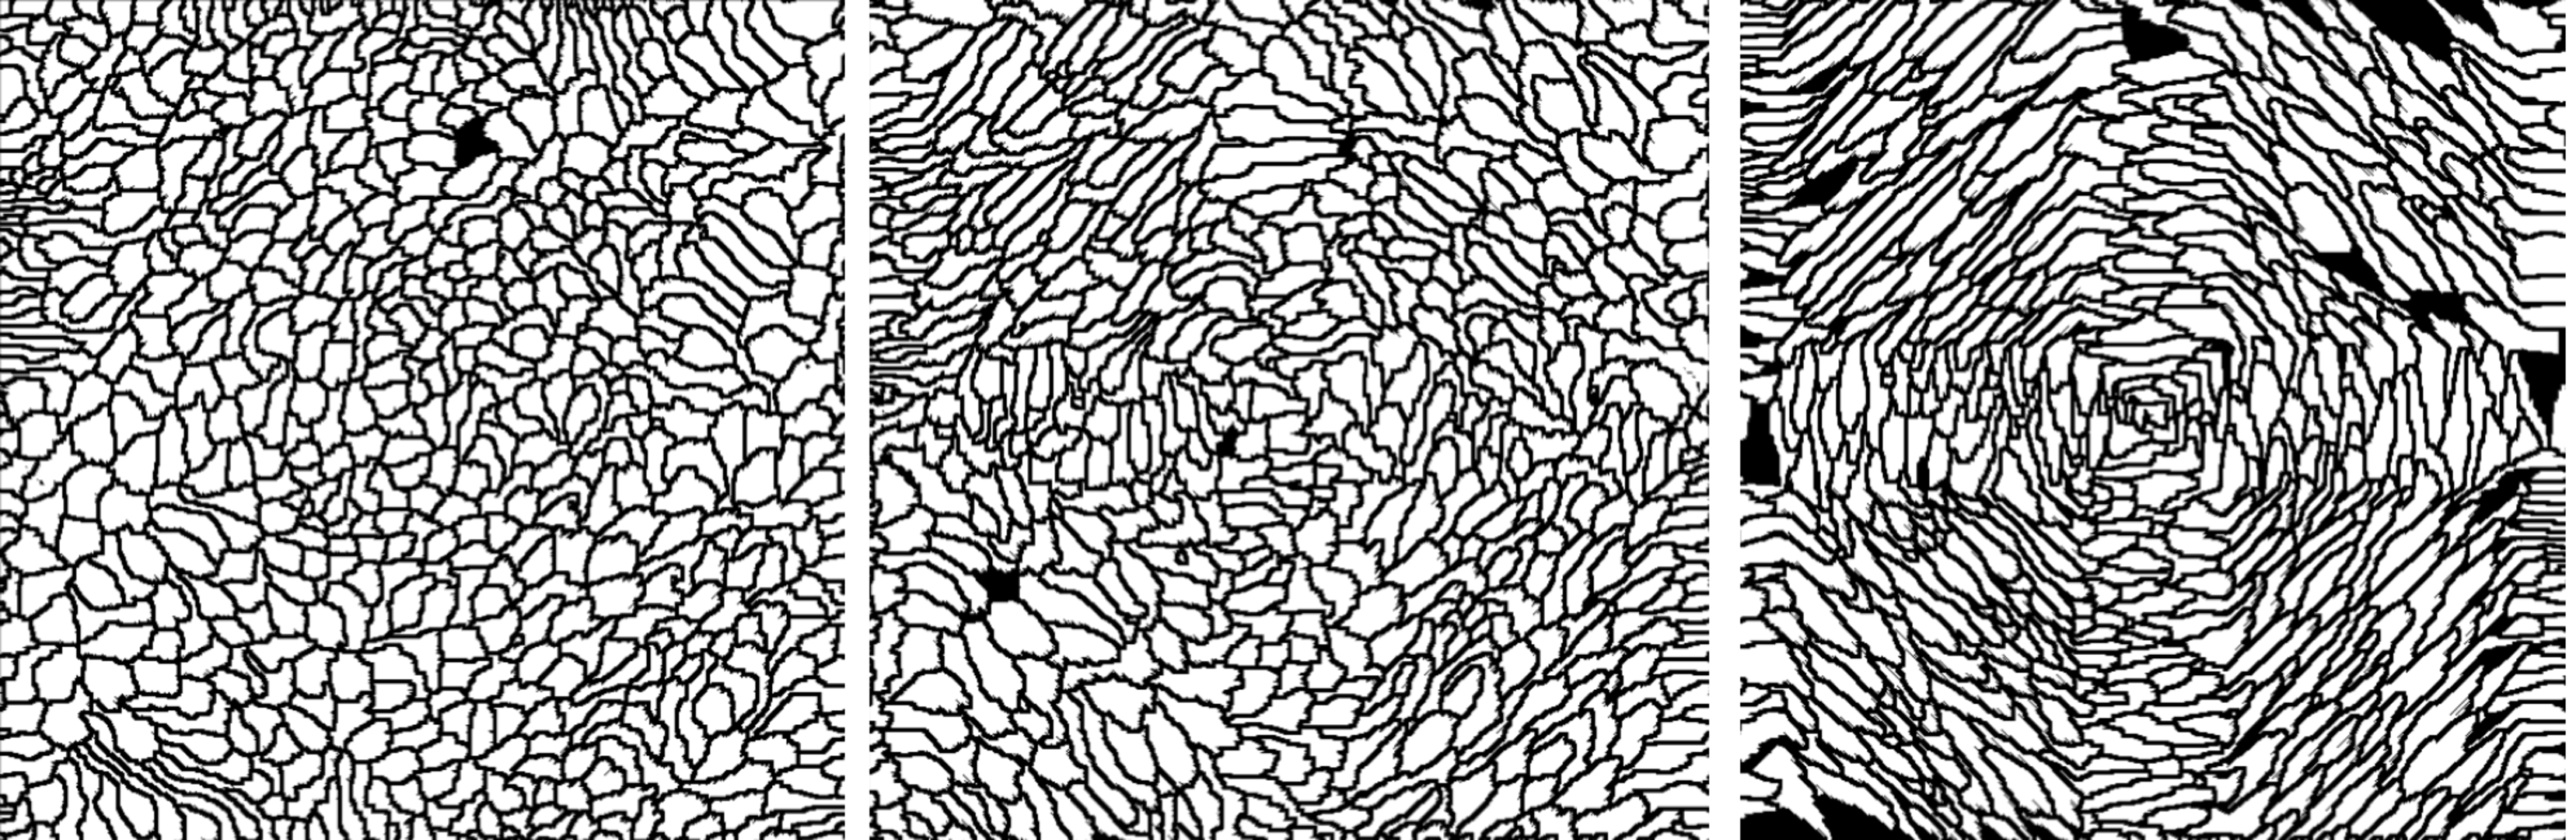
\includegraphics[width=8cm]{../figures/Fig3}

\animategraphics[loop,controls,height=3cm]{12}{../figures/particles/optimised-}{0}{84}
\end{frame}

\begin{frame}{Condiciones de contorno}
Geometrías tridimensionales \textbf{arbitrarias} $\rightarrow$ voxelización

\begin{itemize}
\item Cortes bidimensionales sobre un Eje Cartesiano ($x$, $y$ o $z$)
\item Para cada corte se establecen condiciones de contorno, a través de un campo vectorial discreto que ``sigue'' al contorno (blur (ventana $k$) $\rightarrow$ gradiente $\rightarrow$ ortogonal)
\item Centrado del SD en el {\em centro de masa} de cada corte
\item Parametrización bidimensional (más intuitiva).

\end{itemize}

  \centerline{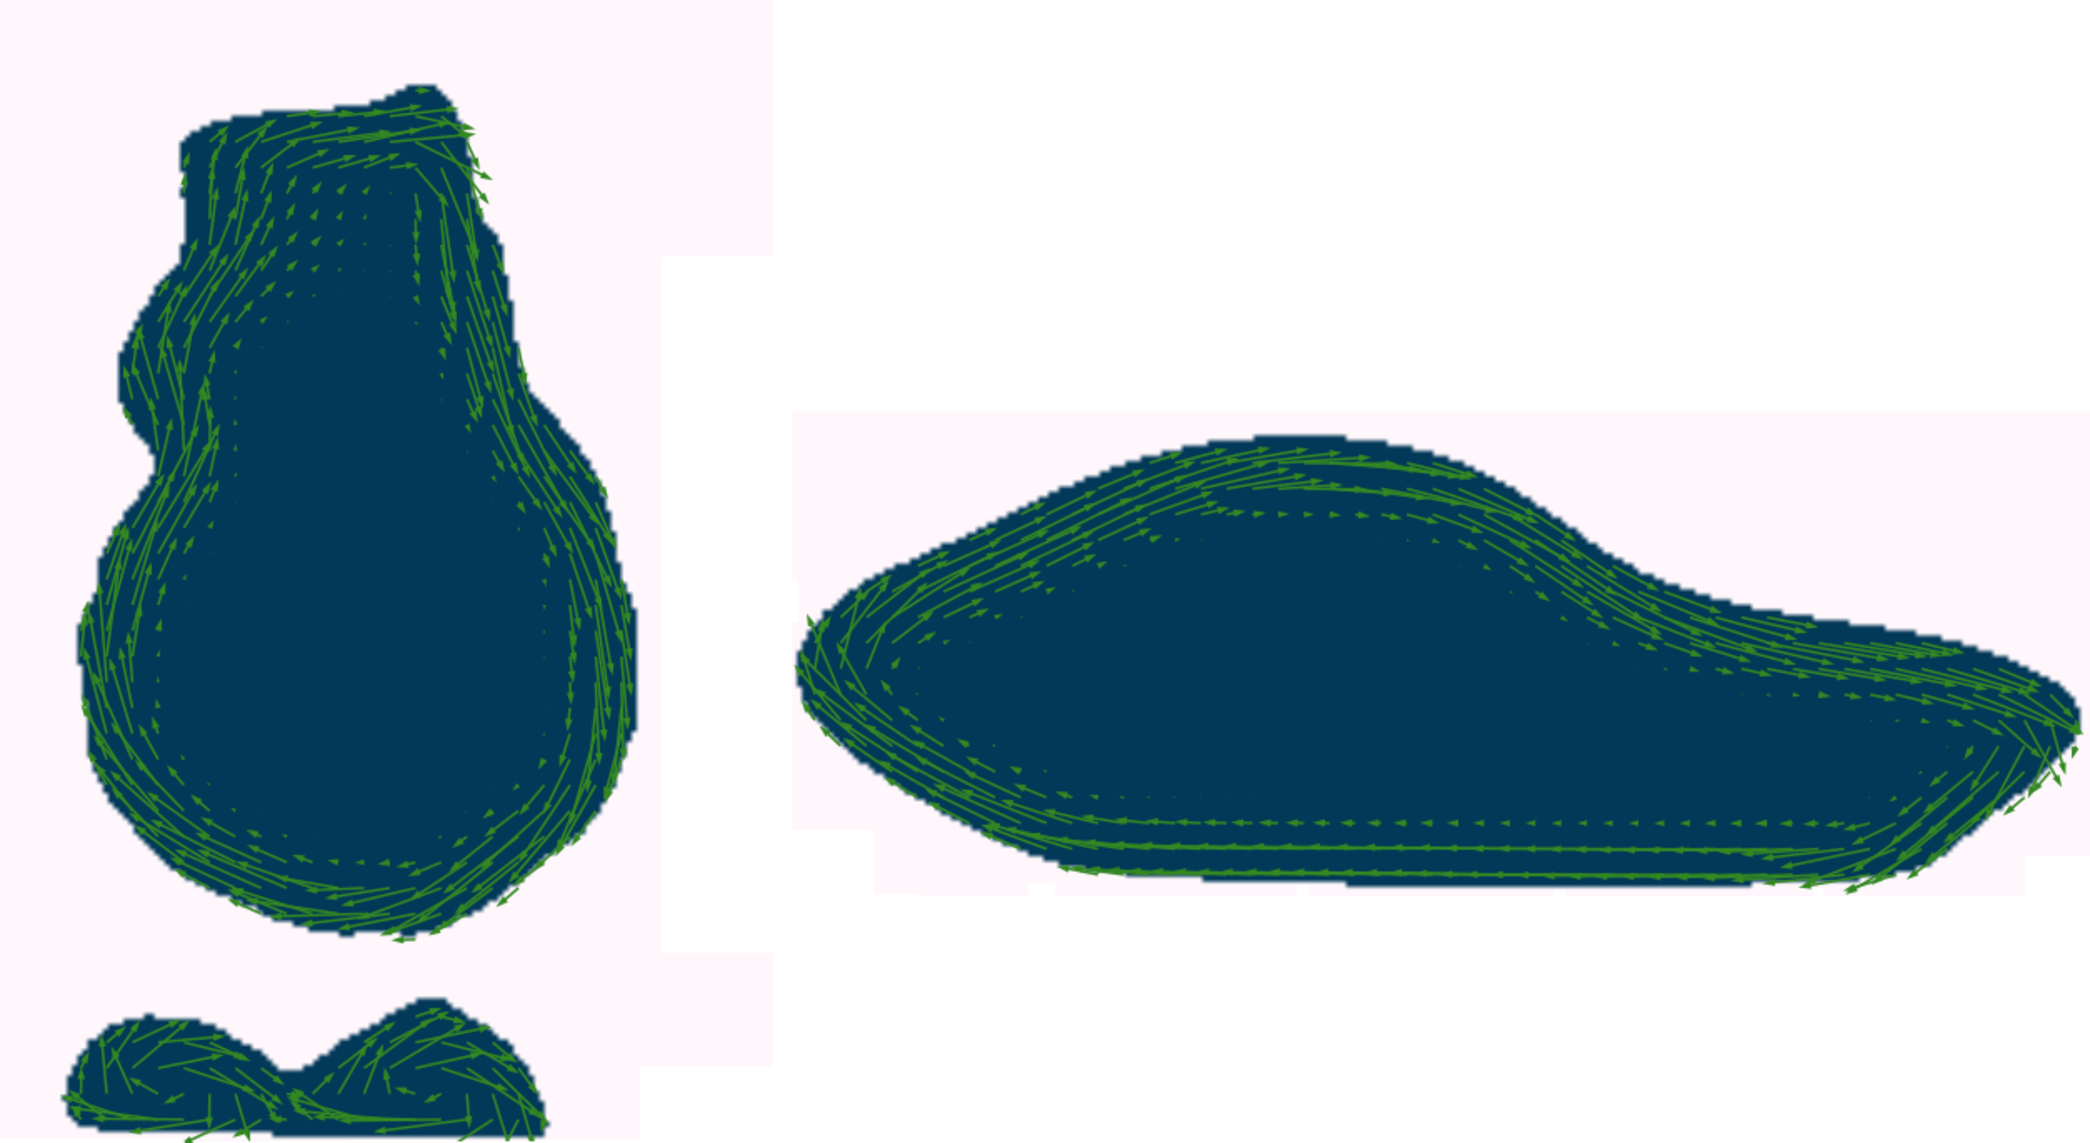
\includegraphics[width=5cm]{../figures/Fig4}}
\end{frame}


\subsection{Resultados}

\begin{frame}{Resultados}
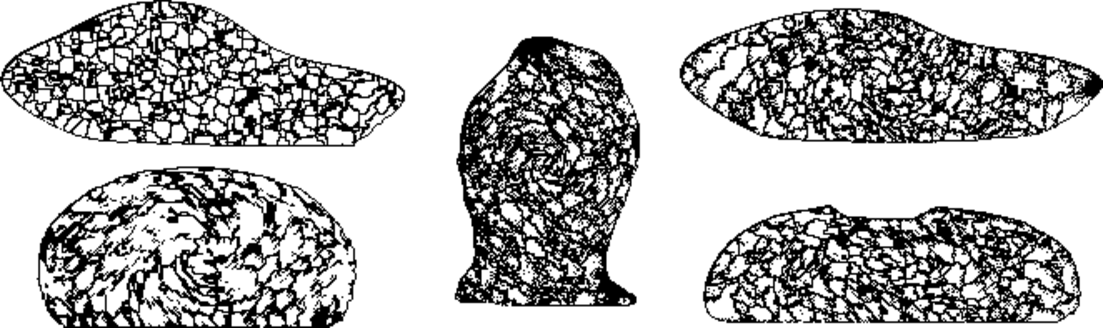
\includegraphics[width=10cm]{../figures/Fig5}

Parámetro {\em separación} = 2 entre partículas, Adaptativo (dependiendo del ancho y alto del corte).

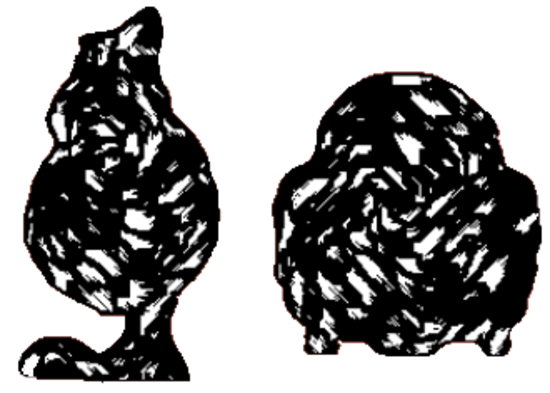
\includegraphics[width=4cm]{../figures/Fig7}
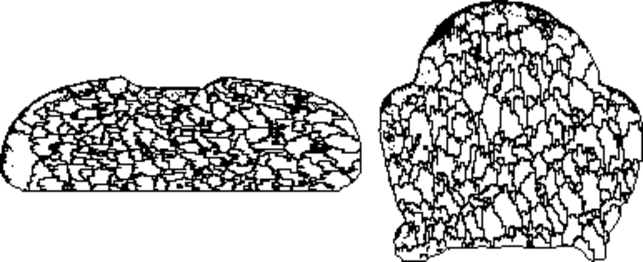
\includegraphics[width=5cm]{../figures/Fig6}





\end{frame}



\begin{frame}{Resultados - Modelado de Materiales Porosos}

\centerline{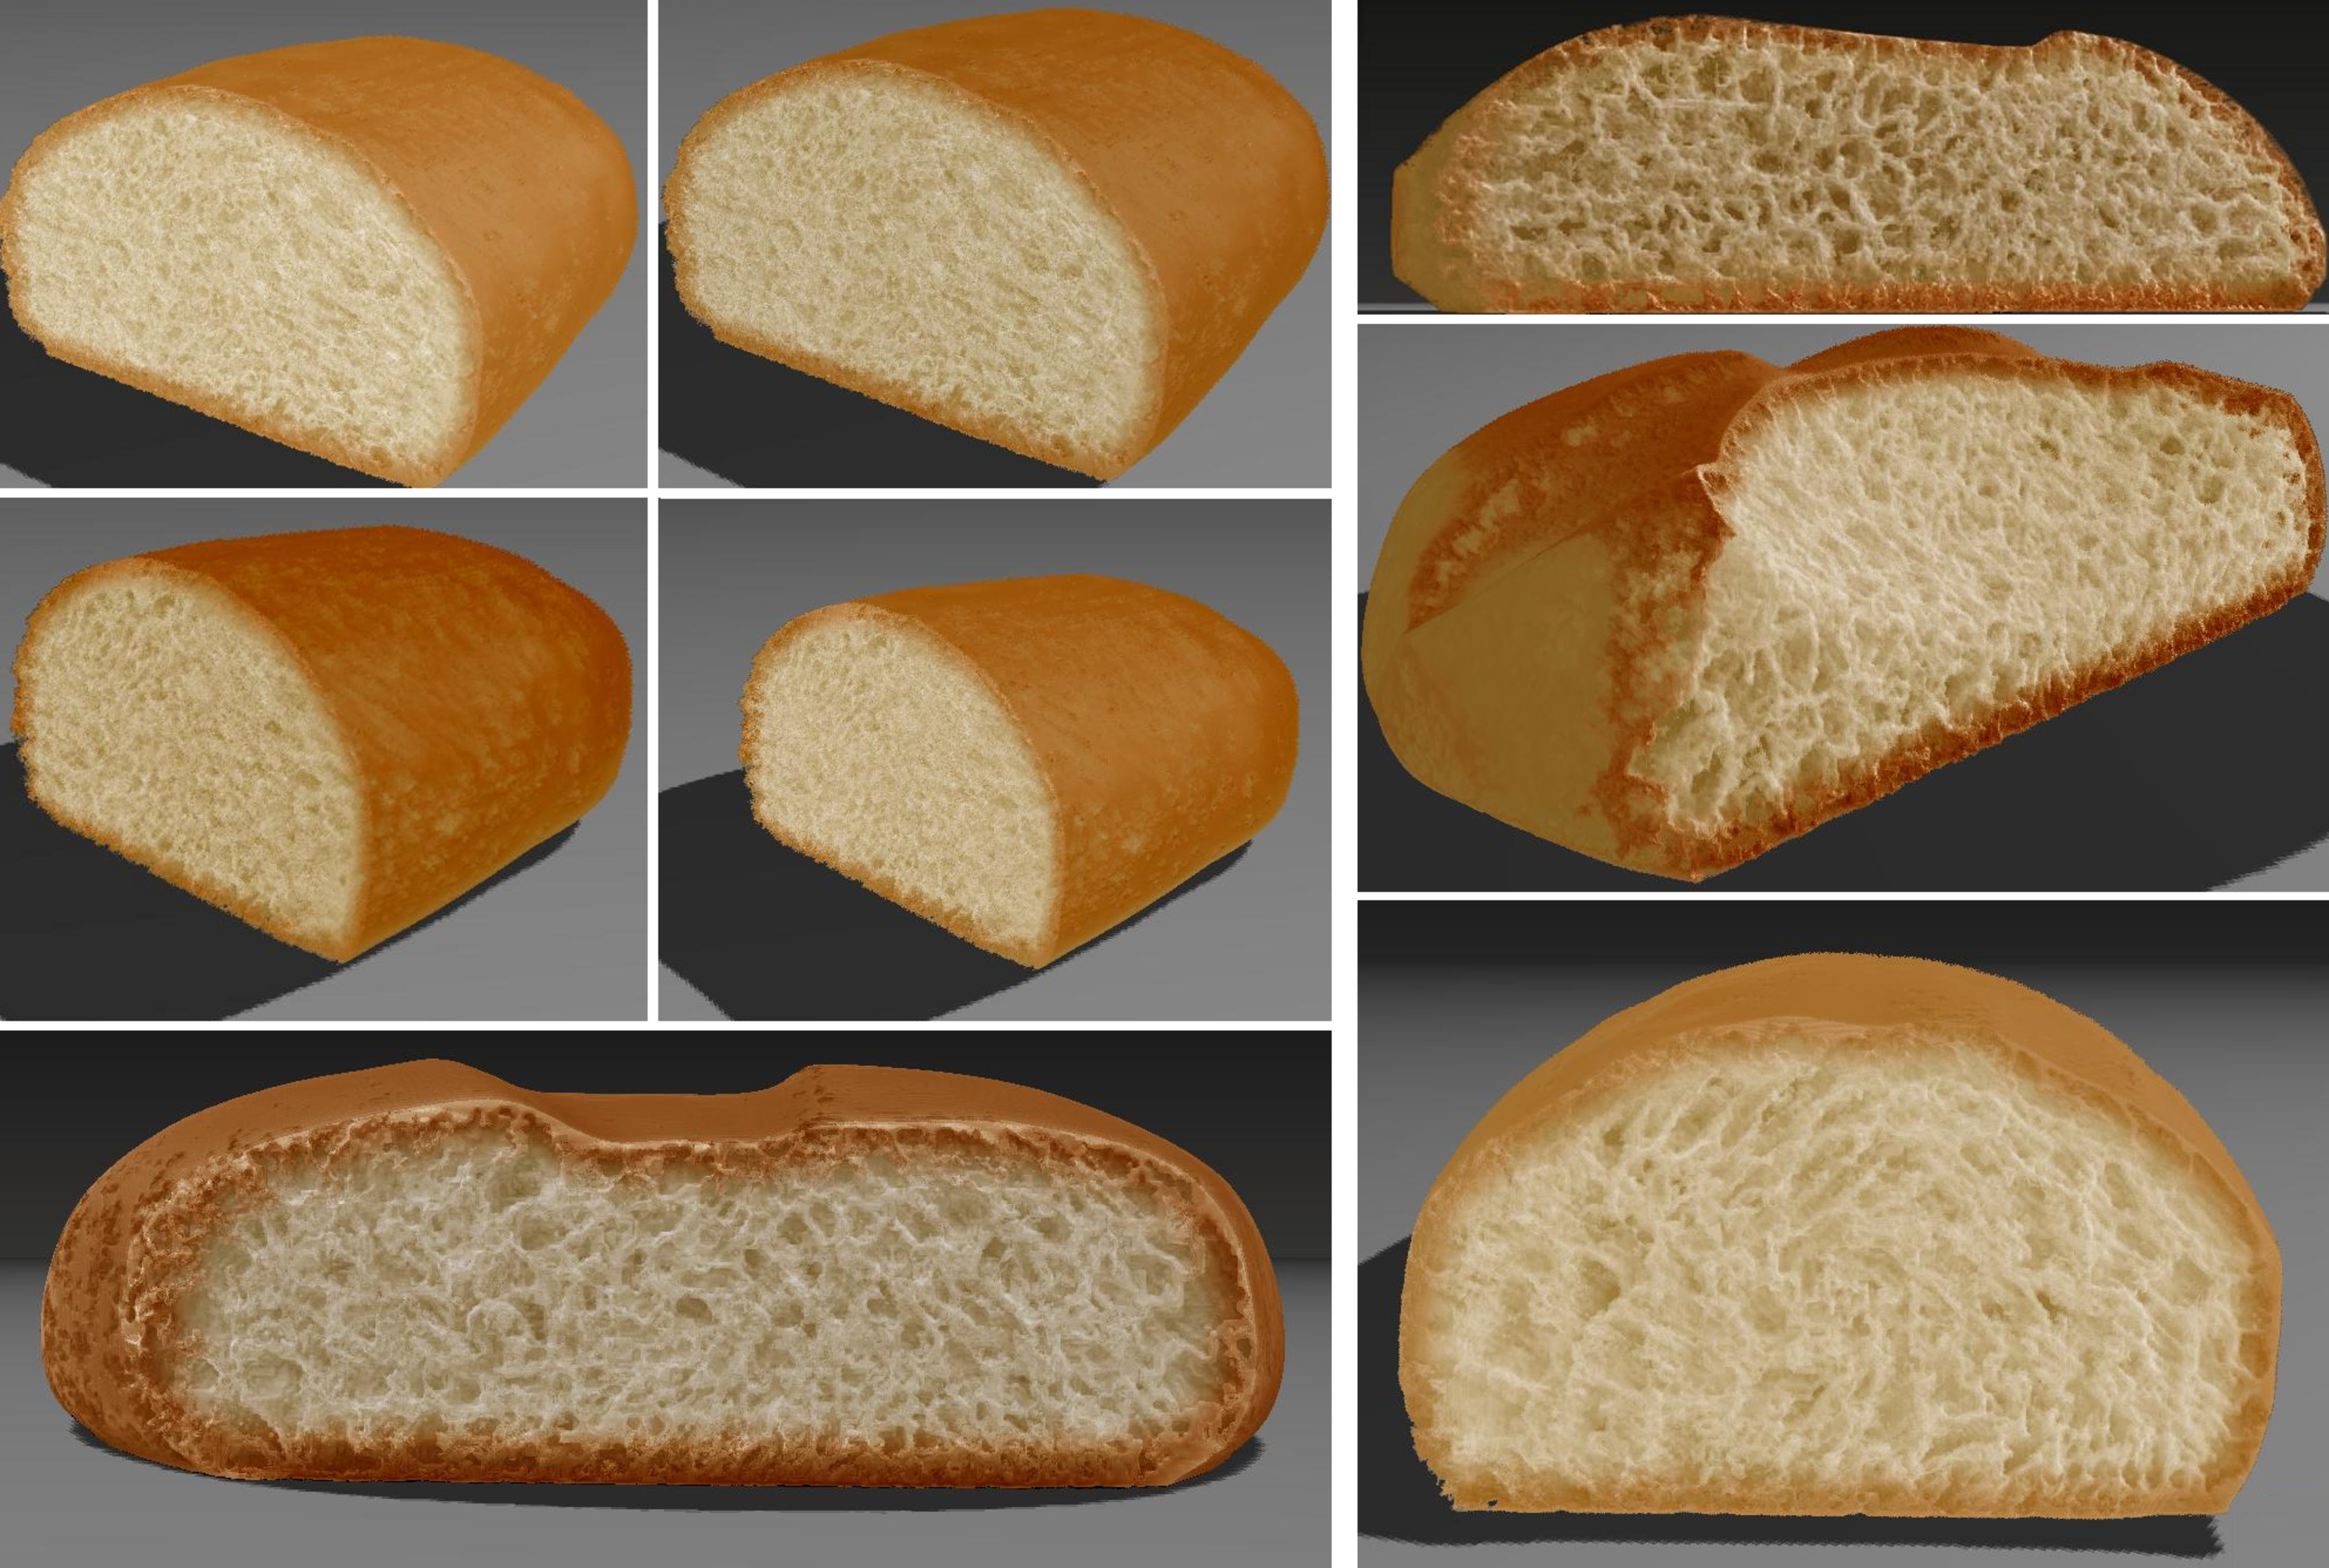
\includegraphics[width=9.5cm]{../figures/Fig12CAVW}}
\end{frame}

\begin{frame}{Resultados - Modelado de Materiales Porosos}

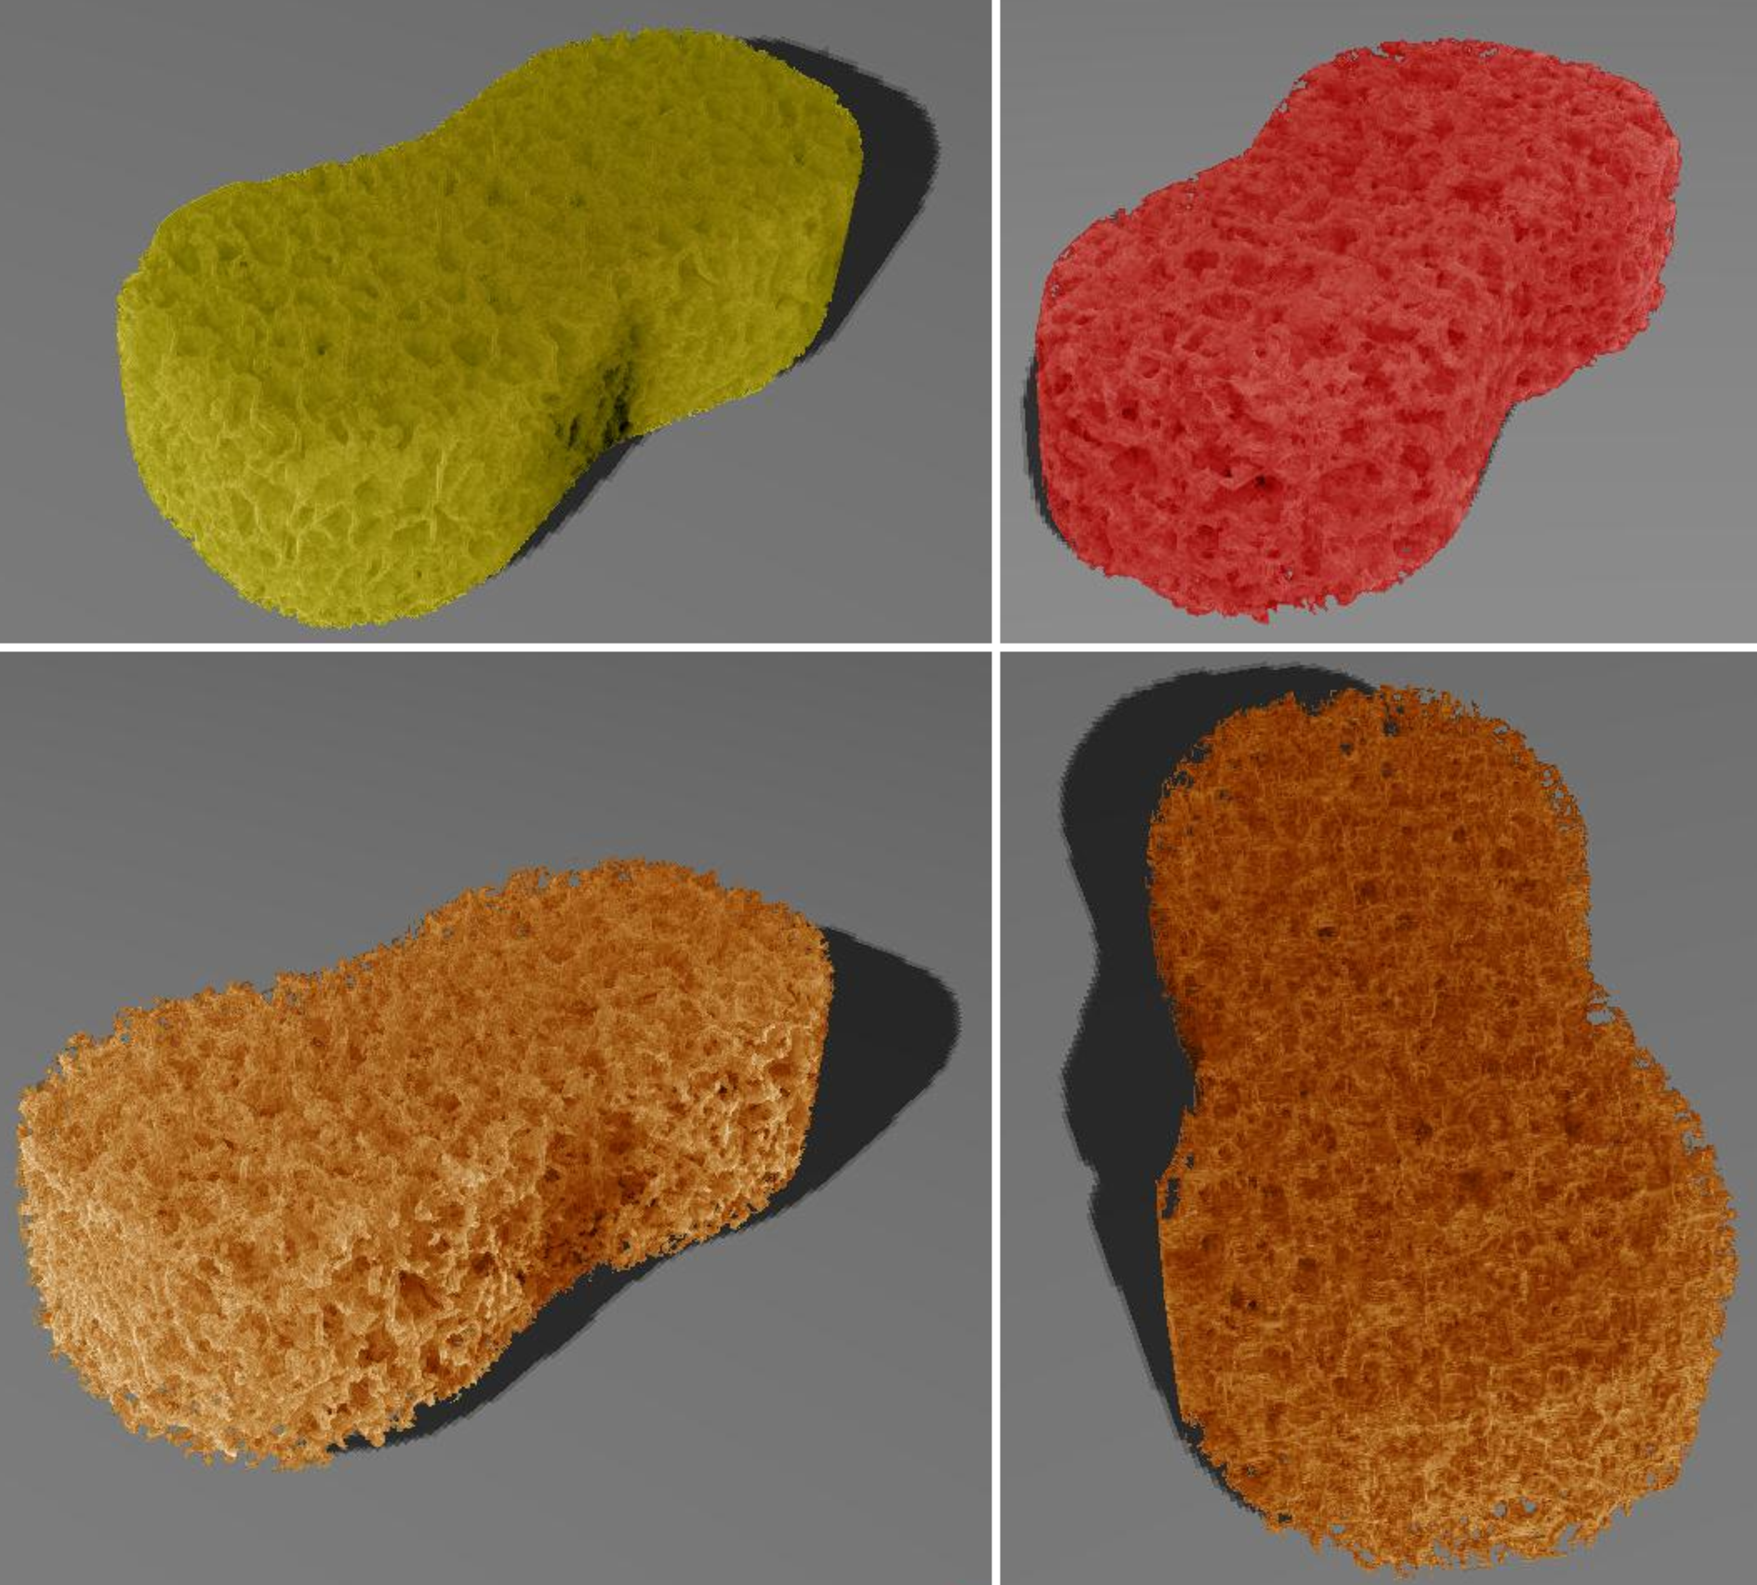
\includegraphics[width=6cm, height=5cm]{../figures/Fig13CAVW}
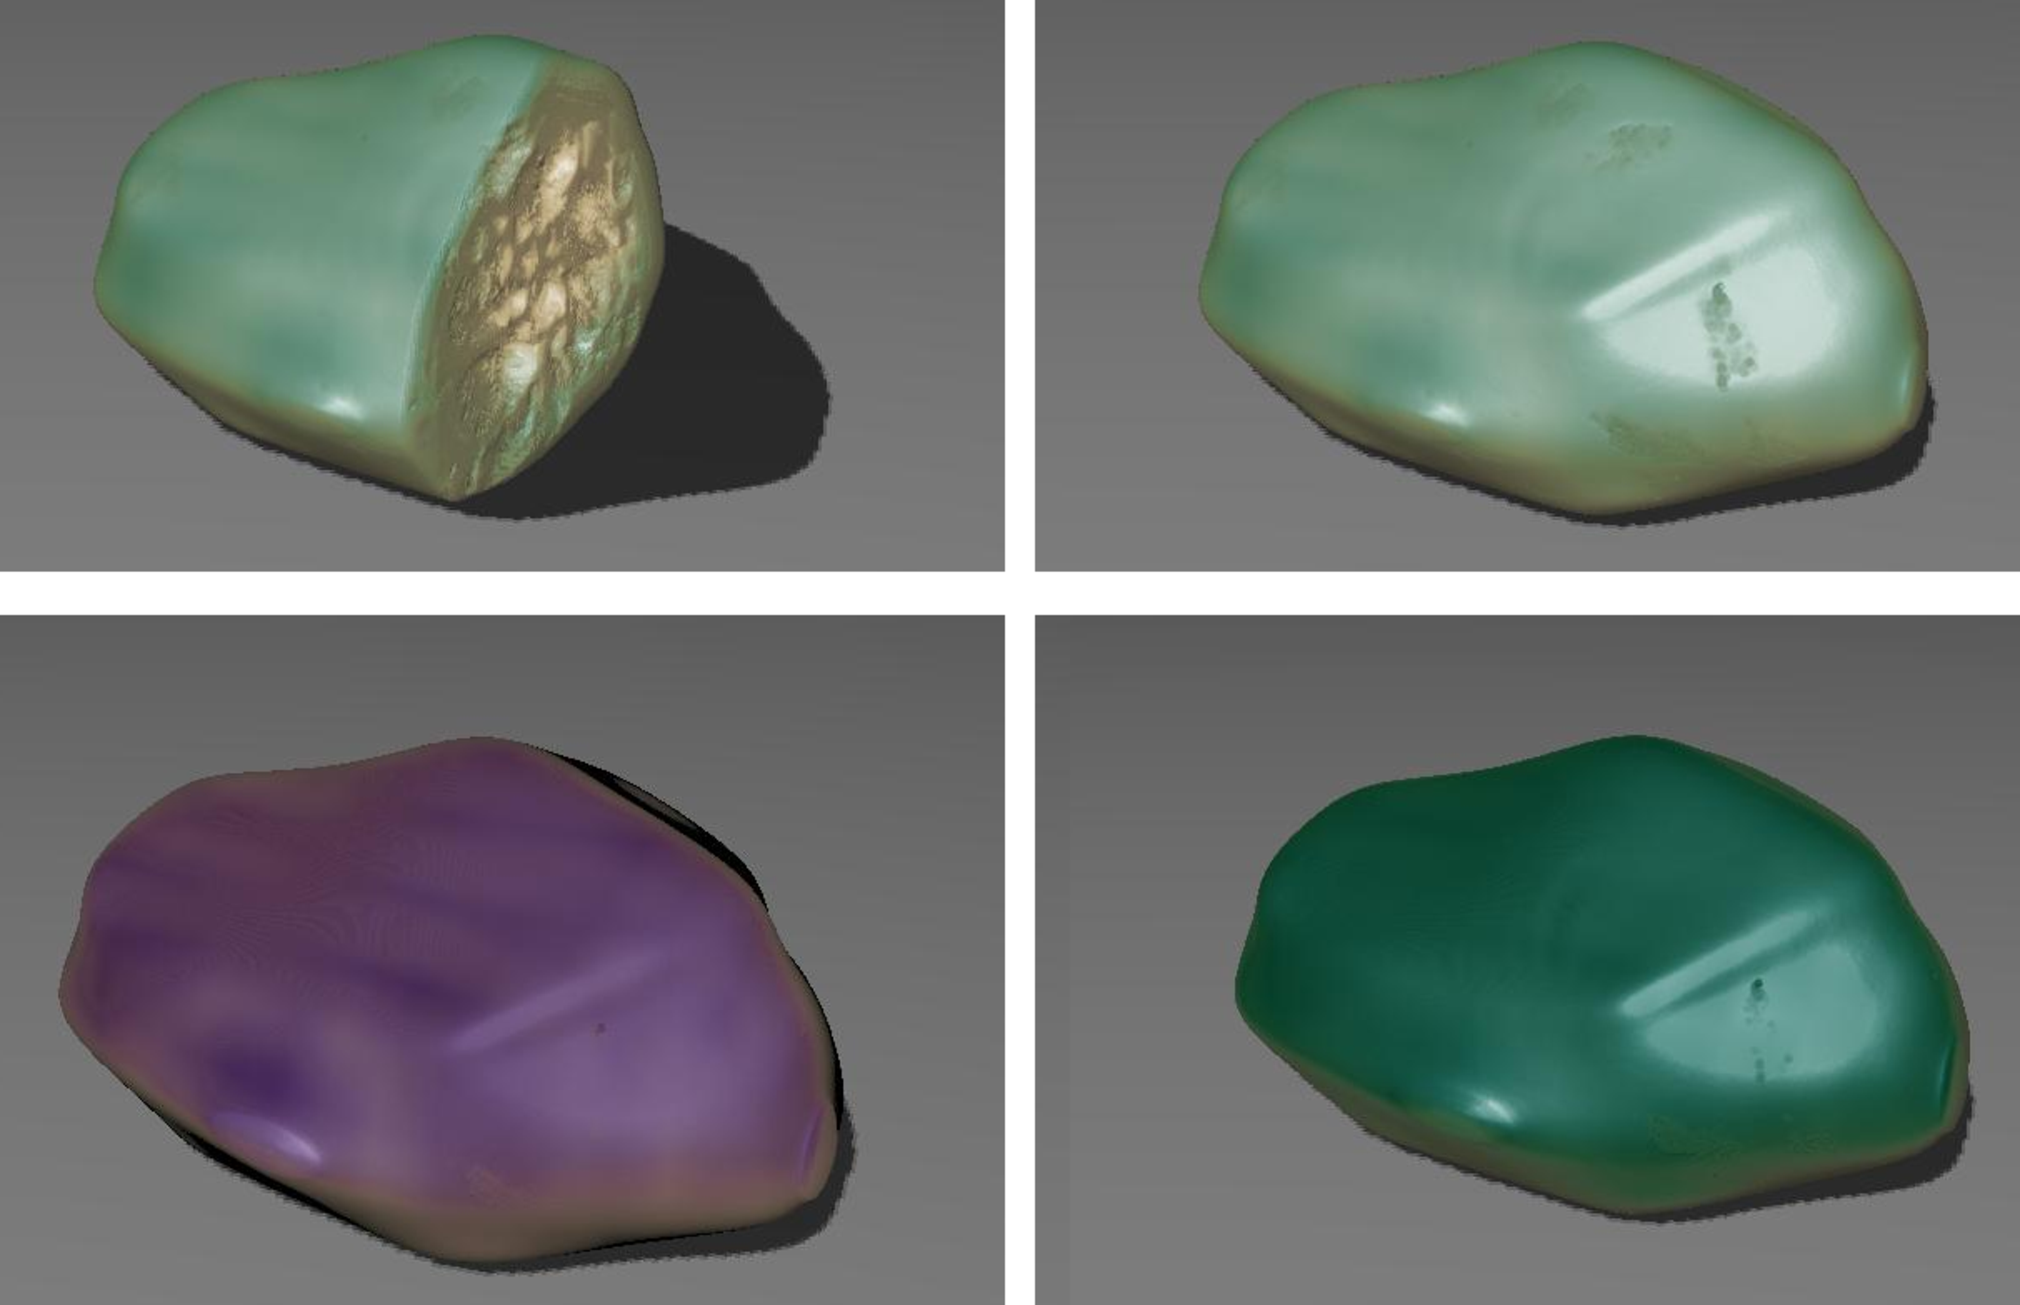
\includegraphics[width=6cm, height=5cm]{../figures/Fig14CAVW}

\end{frame}


\begin{frame}{Conclusiones\footnote{Realistic Modeling of Porous Materials, {\it J. Computer Animation and Virtual Worlds}, Baravalle et.al. 2016}}
\begin{block}{}
\begin{itemize}
\item Algoritmo procedimental fenomenológico
\item Resultados adecuados para computación gráfica
\item Permite representar diversos materiales porosos
\item No requiere esfuerzo por parte del usuario

\item Dificultad al controlar los sistemas dinámicos
\end{itemize}
\end{block}
\end{frame}


\section[Modelado de Pan]{Modelado procedimental de pan inspirado en su proceso de formación}


\begin{frame}
\begin{block}{}
\begin{center}
\vspace{1cm}
\huge{Modelado procedimental de pan inspirado en su proceso de formación}
\vspace{1cm}
\end{center}
\end{block}
\end{frame}

\subsection{Modelado procedimental de pan inspirado en su proceso de formación}
\begin{frame}{Modelado procedimental de pan inspirado en su proceso de formación}
\begin{block}{}
\begin{itemize}
\item Ignorado en gran medida en la literatura de computación gráfica, ha sido ampliamente estudiado en ingeniería de los alimentos.
\item No existe aún un modelo unificado (cocción, leudado, formación de la corteza, etc.).
\end{itemize}
\end{block}

\centerline{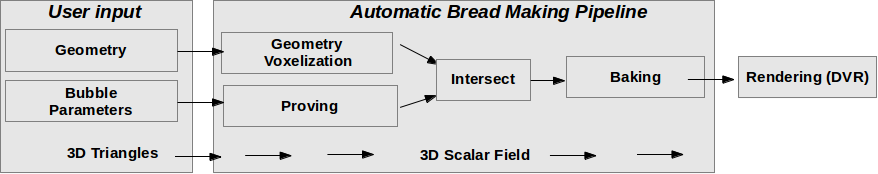
\includegraphics[width=10cm]{../figures/pipeline}}
\end{frame}

\begin{frame}{Leudado}
Simulación por \textbf{extracción de esferas} de un cubo

$N(r)$: cantidad de esferas extraídas (inversamente proporcional al radio $r$ de la esfera). Ley fractal:

\begin{equation*}
N(r) = \frac{k}{r^{d}}
\end{equation*}

\vspace{0.3cm}
Sintético \hspace{2.1cm} Real \hspace{2.6cm} Real
\centering
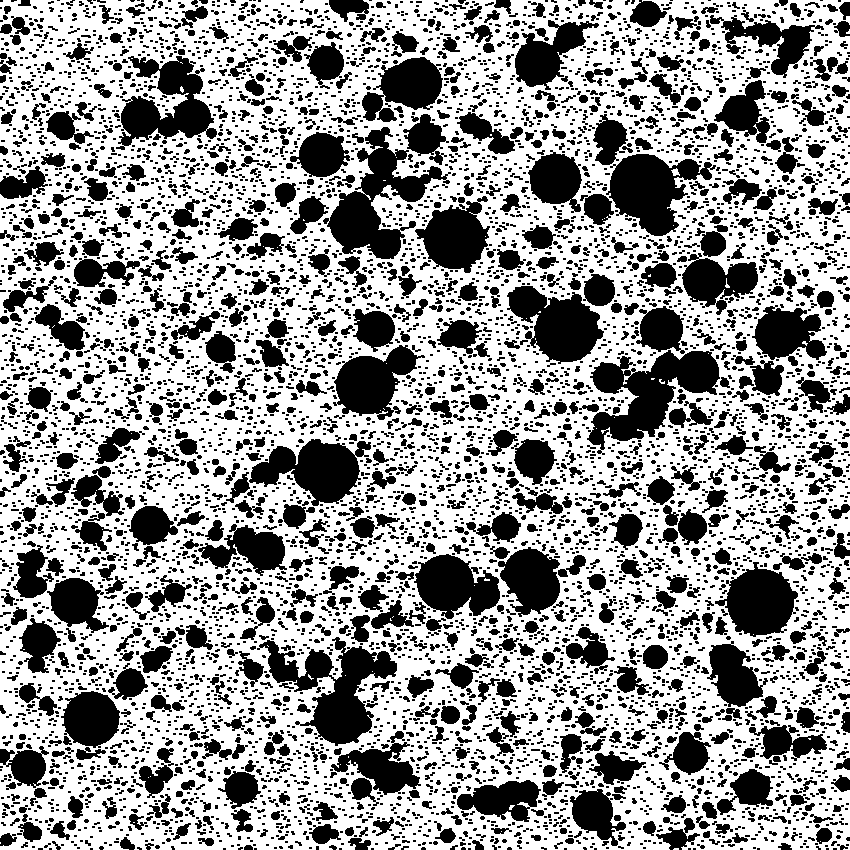
\includegraphics[height=3.5cm]{../figures/bubbles}
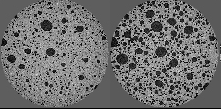
\includegraphics[height=3.5cm]{../figures/proving}

\end{frame}

\begin{frame}{Resultados - Proceso formación Pan}
\textbf{Mapa de Distancias}
\centerline{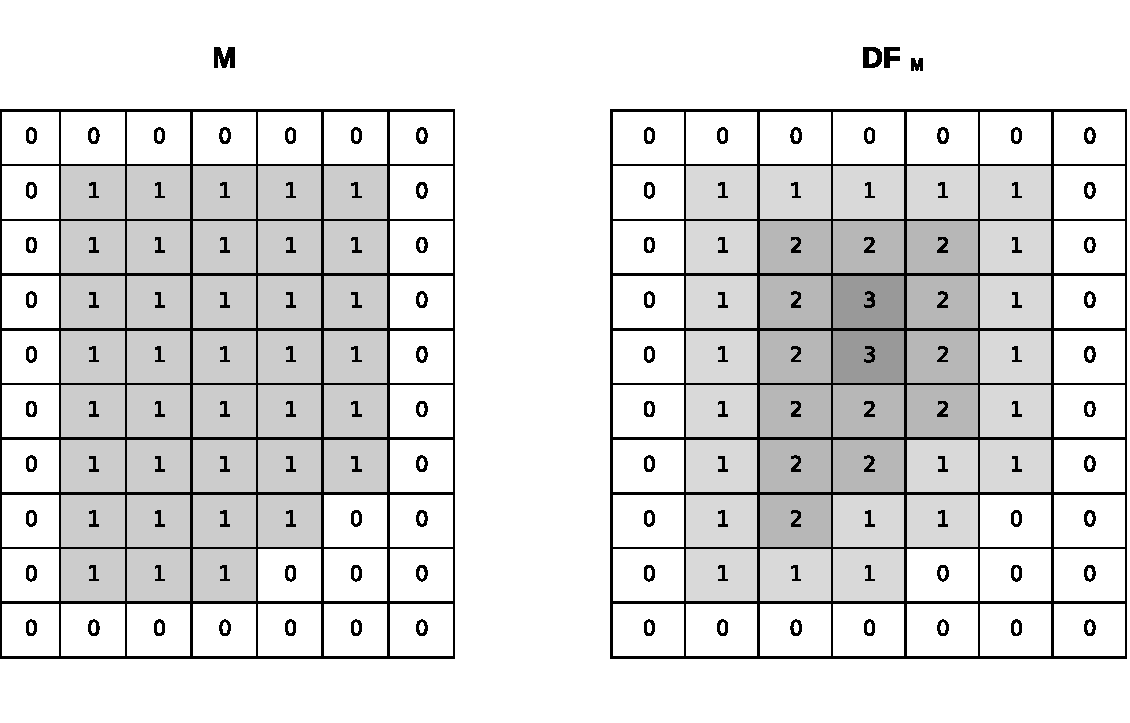
\includegraphics[width=4cm]{../figures/DistanceTransform}}

\textbf{Umbral} DF $\rightarrow$ corteza de ancho \textbf{parametrizable}.

\vspace{0.3cm}

\centerline{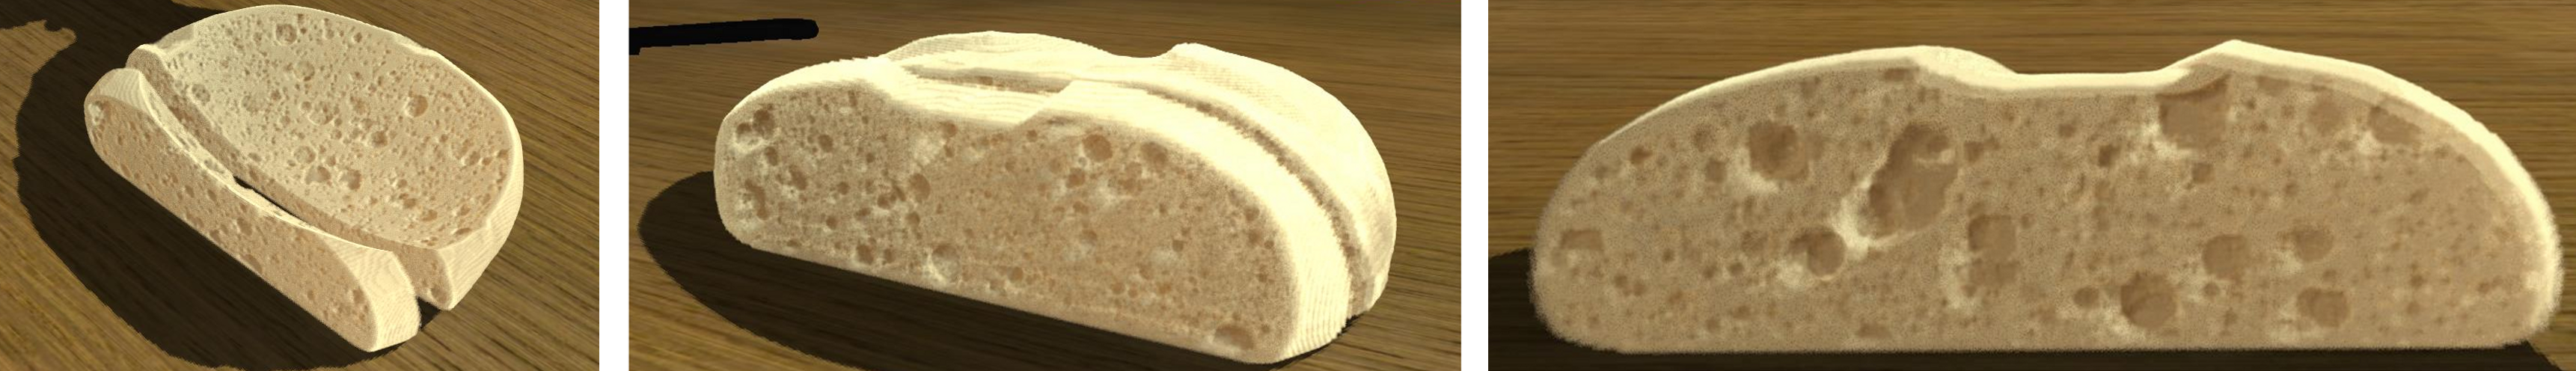
\includegraphics[width=8cm]{../figures/prebakebread}}

\centerline{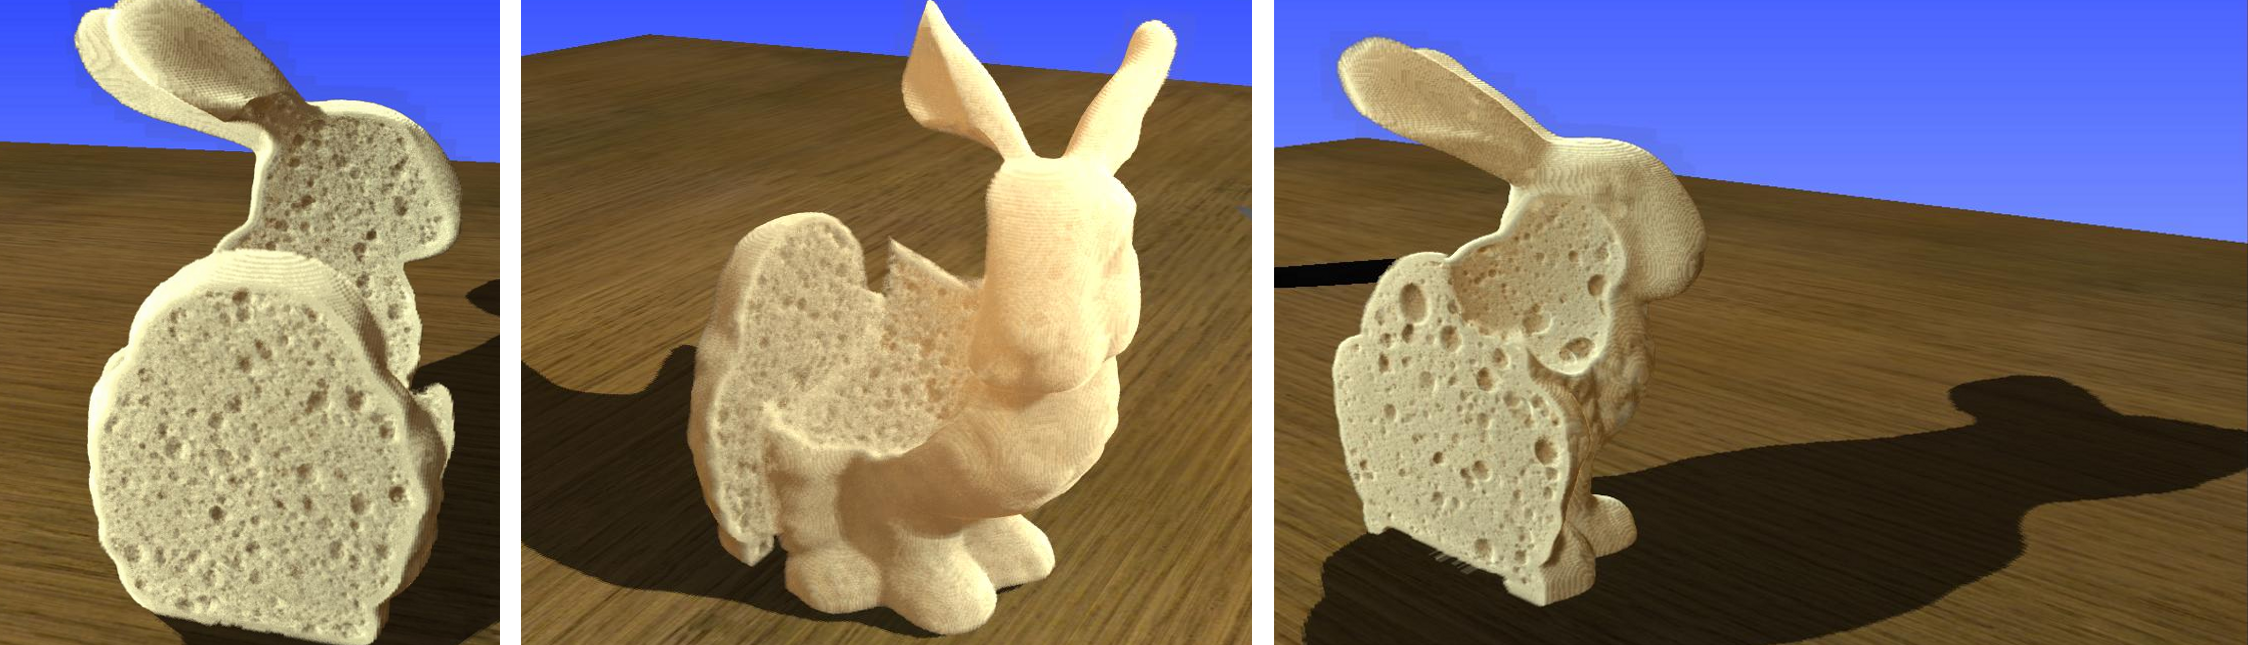
\includegraphics[width=8cm]{../figures/prebakebunny}}
\end{frame}


\subsection{Cocción}

\begin{frame}{Cocción}
Utilizamos un Modelo $1D$:
\begin{itemize}
\item Se busca \textbf{Deformación por Temperatura}
\item Soluciones similares para nuestros propósitos (apariencia creíble)
\end{itemize}

$Temp$: Arreglo \textbf{unidimensional} de temperaturas.

Distribución 3D de la temperatura
\begin{equation*}
\displaystyle R_{vol}[x,y,z] = Temp[ round( DF_{M}[x,y,z] ) ], 
\end{equation*}

$DF_{M} = 0 \rightarrow$ contorno, mayor $T$ $Temp[0] \rightarrow R_{vol}$

$DF_{M} > 0 \rightarrow$ interior, menor $T$  $\rightarrow R_{vol}$

\centerline{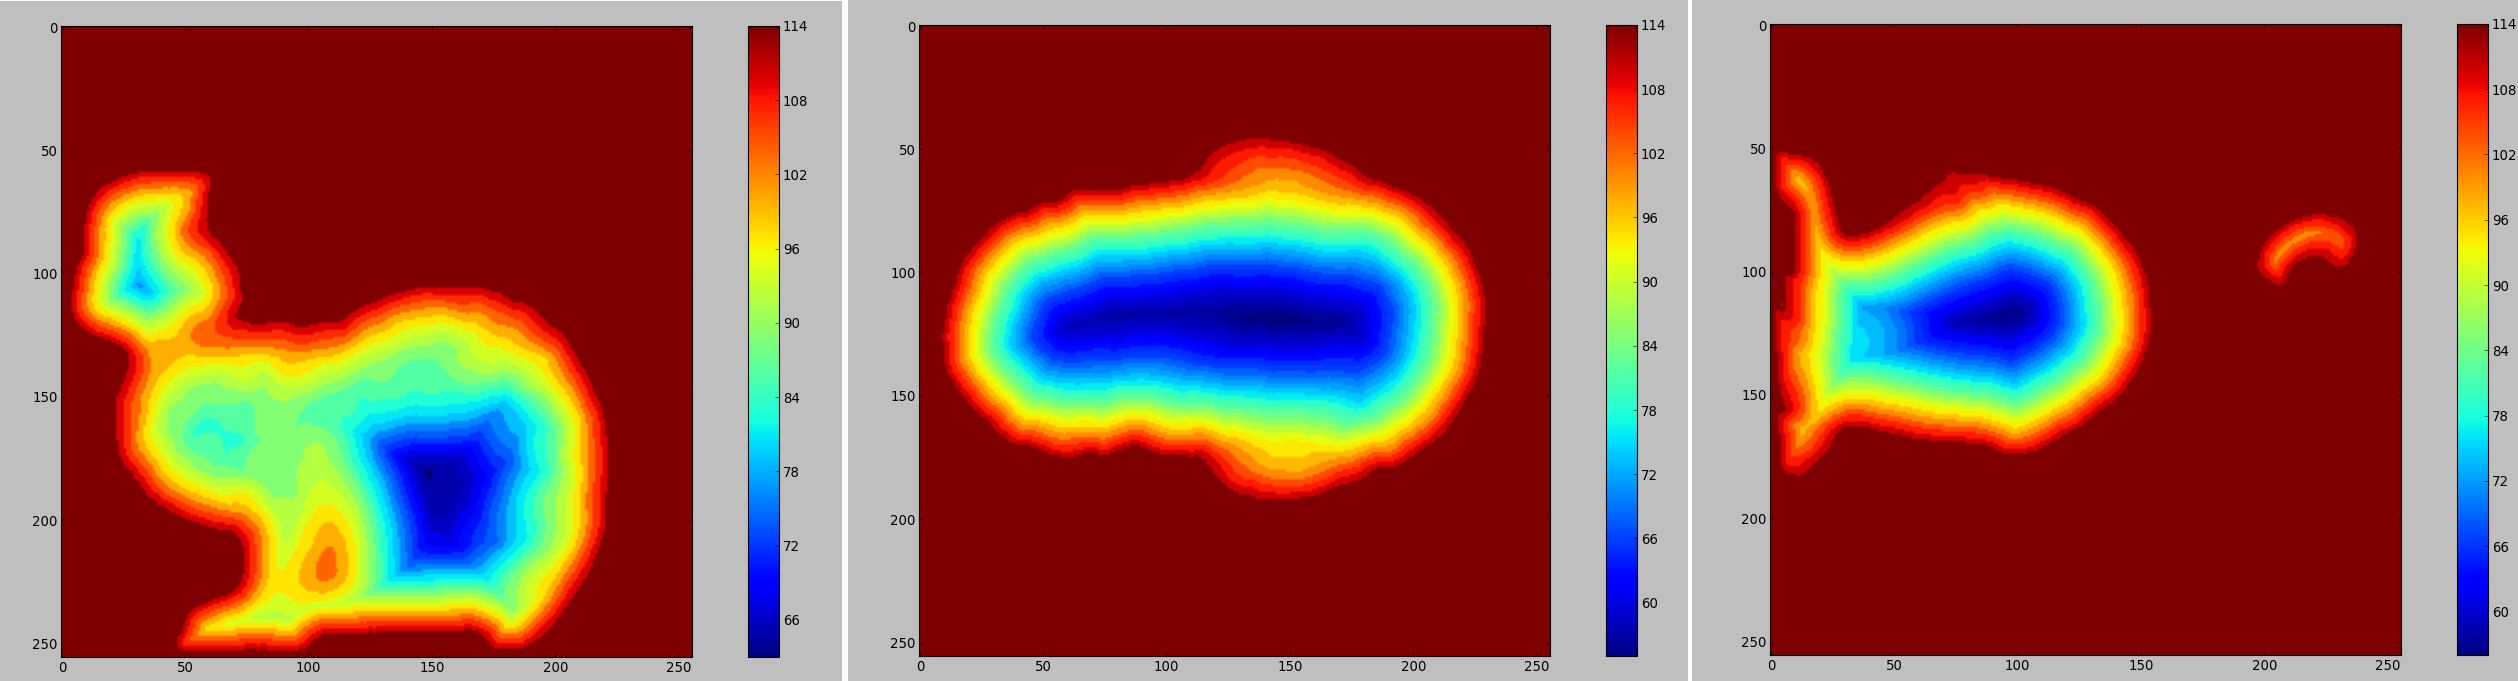
\includegraphics[width=8cm]{../figures/tempsbunny}}
\end{frame}

\begin{frame}{}
\textbf{Deformación por Temperatura} - \textbf{Warping}


\textbf{Burbujas} durante el leudado $\rightarrow P[x,y,z] = max \bigg\{r\bigg\}$

\begin{equation*}
[r,s,t] = [u,v,w] + P[u,v,w] \, \nabla R_{vol}[u,v,w],
\end{equation*}

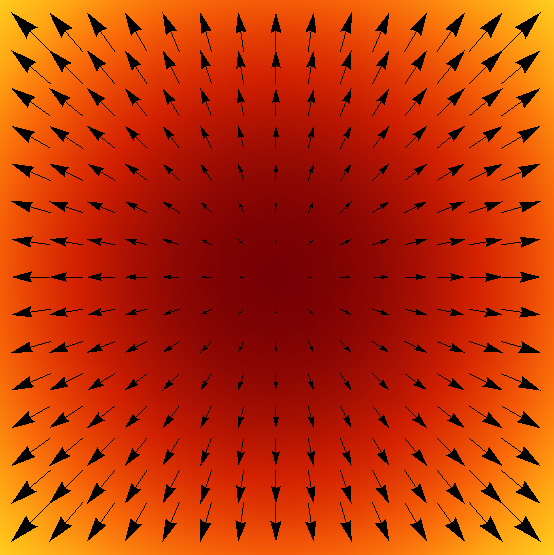
\includegraphics[width=2.2cm]{../figures/gradient}
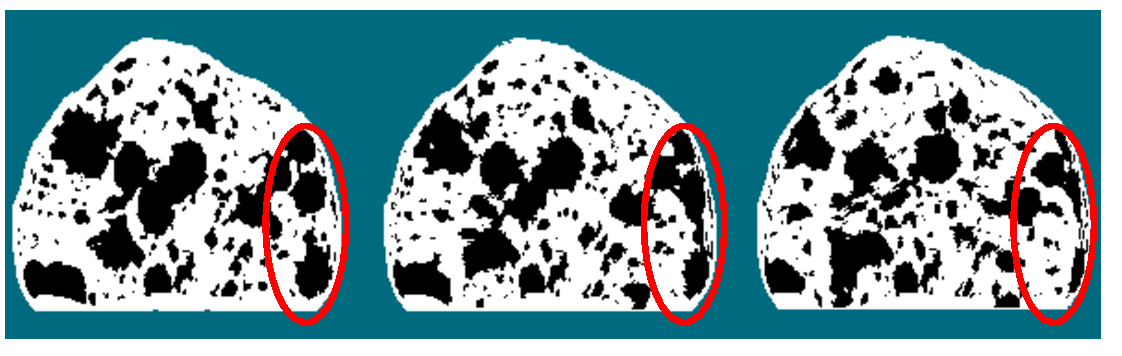
\includegraphics[width=7cm]{../figures/parameterp}

Escalado de la textura (distribución de burbujas)

\begin{equation*}
[x,y,z] = [r,s,t]\, S \, P[r,s,t],
\end{equation*}

\end{frame}

\begin{frame}{Resultados}

\centerline{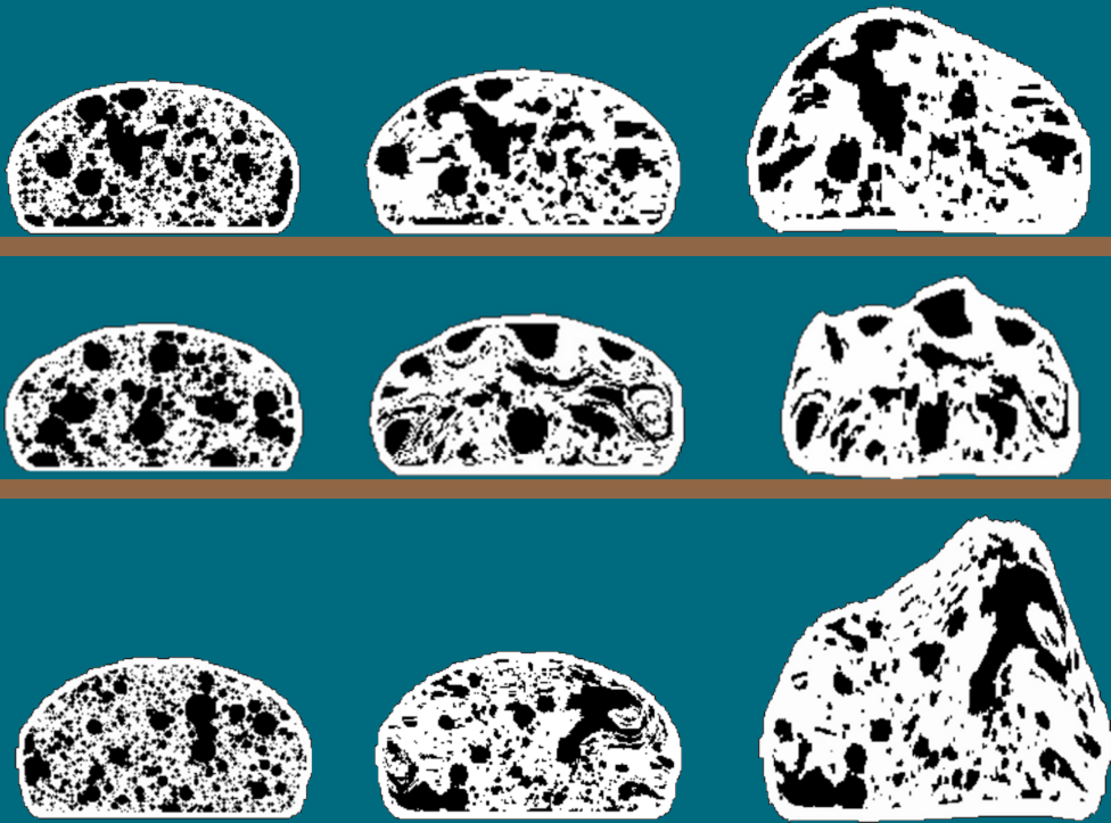
\includegraphics[width=9cm]{../figures/Fig9}}

\end{frame}

\begin{frame}{Resultados - Proceso formación Pan}

\centerline{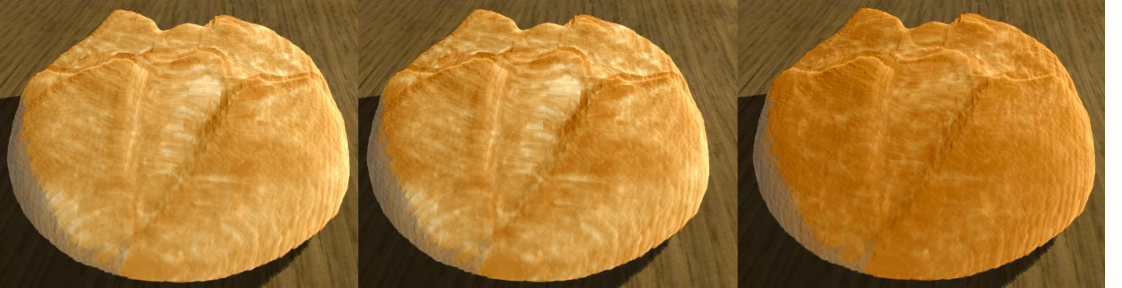
\includegraphics[width=8cm]{../figures/Fig13}}
Cortezas con diferentes historias de cocción ($L_{MAX}$).

\vspace{0.2cm}

Colores CIELab (Luminancia, Cromaticidad) de muestras reales (Purlis et. al. (2009))

\vspace{0.2cm}

$L = 40 \rightarrow$ \text{máxima cocción}, $L = 90 \rightarrow$ \text{sin cocción}

\vspace{0.2cm}

\centerline{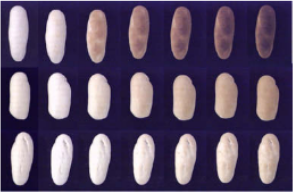
\includegraphics[width=2cm]{../figures/browning}}

%{\em \textbf{Densidad} de la corteza}: $N_{v} / W_{size} \rightarrow L$

%\begin{itemize}
%\item $N_{v}$ núm. voxels $= 1$ en una ventana en el entorno de la posición,
%\end{itemize}

$<$ masa $\Rightarrow < L$.

\end{frame}

\begin{frame}{Resultados - Proceso formación Pan}
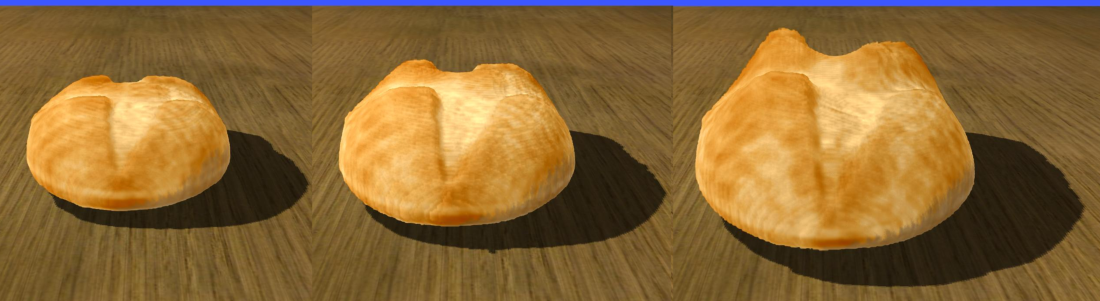
\includegraphics[width=10cm]{../figures/Fig14}

Panes luego de la cocción mostrando diferentes crecimientos. De izquierda a derecha se incrementa el parámetro $S$.

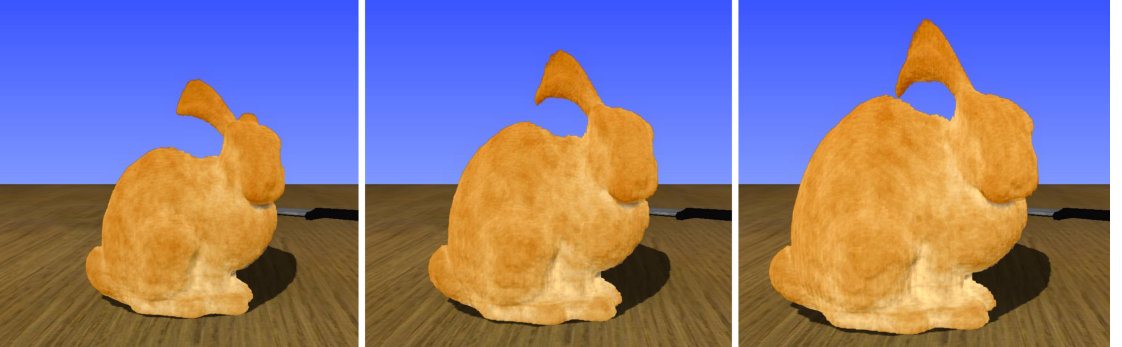
\includegraphics[width=7cm]{../figures/Fig15}


\end{frame}


\begin{frame}{Validación}

Ley fractal $\rightarrow$ geometrías de migas de pan.

\begin{block}{Espectro Multifractal (MFS)}

\begin{itemize}
\item \textbf{Vector}, captura distintas estructuras fractales dentro del mismo objeto
\item Computa distintas medidas fractales: información, box-count, correlación, etc.
\end{itemize}
\end{block}

\vspace{0.2cm}

$N$ muestras reales del mismo tipo de pan $\rightarrow MFS_{real}$

$N$ muestras sintéticas $\rightarrow MFS_{sint\acute{e}tico}$, para ciertos parámetros del leudado

\vspace{0.2cm}

\textbf{Métrica de error}:

\begin{equation*}
Error = \displaystyle \sum_{i} abs(mediana_{i}(MFS_{real})-mediana_{i}(MFS_{sint\acute{e}tico})).
\end{equation*}

\end{frame}

\begin{frame}
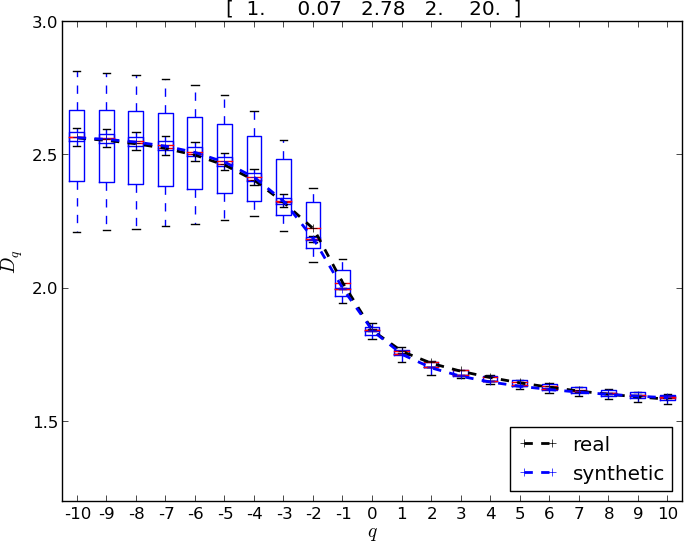
\includegraphics[width=4cm]{../figures/bestboxplot}
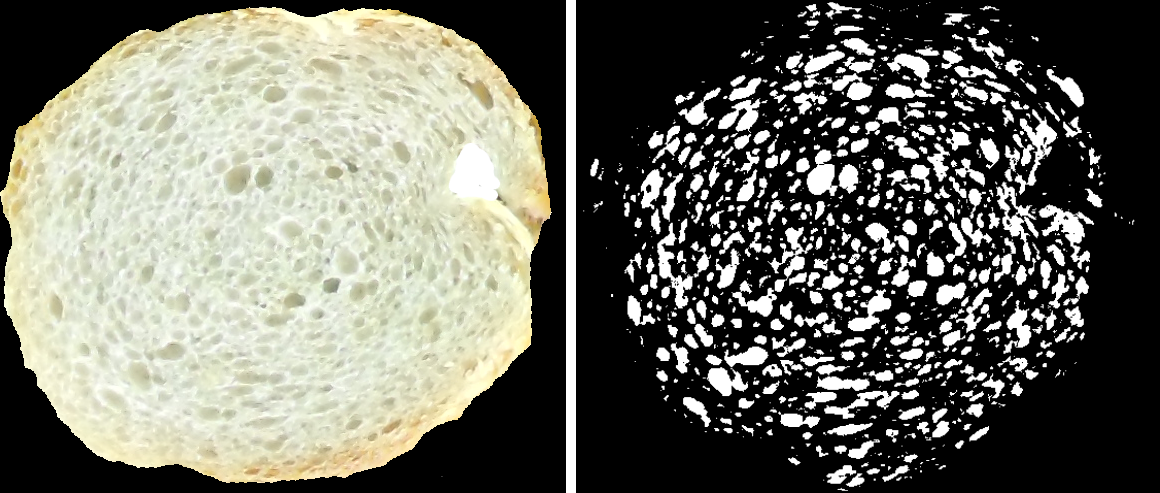
\includegraphics[width=4.5cm]{../figures/realbin}
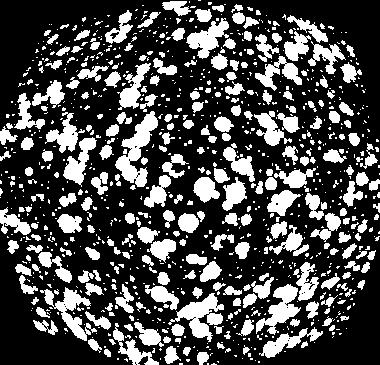
\includegraphics[width=2cm]{../figures/best}

\hspace{4.7cm} Real \hspace{0.6cm} Binarización \hspace{0.5cm} Sintético

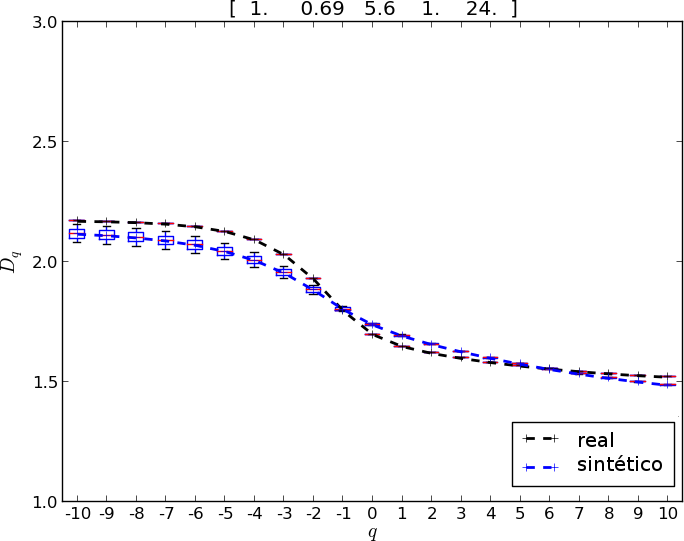
\includegraphics[width=4cm]{../figures/bestboxplot2}
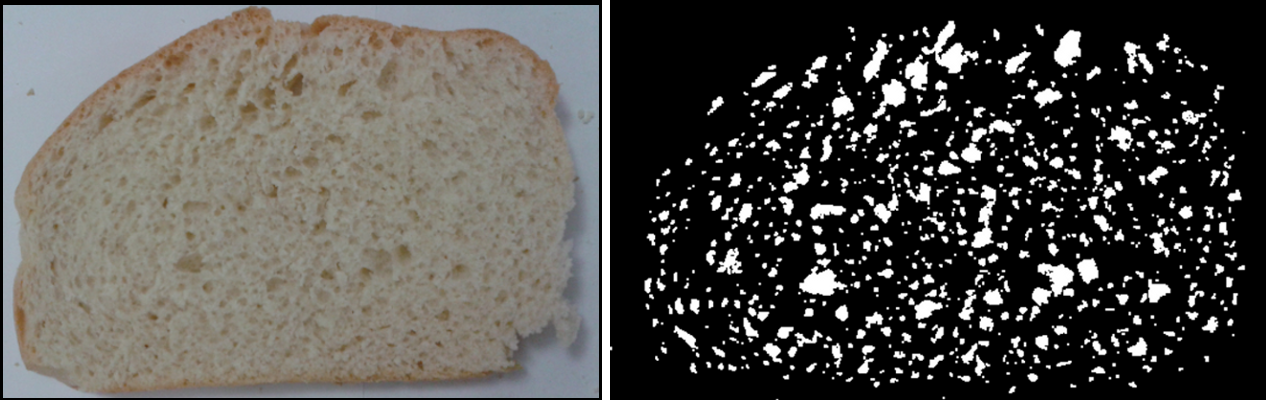
\includegraphics[width=4cm]{../figures/realbin2}
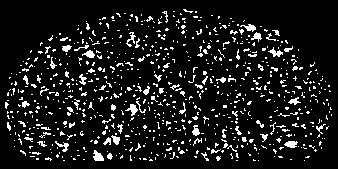
\includegraphics[width=2.5cm]{../figures/best2}

\hspace{4.7cm} Real \hspace{0.5cm} Binarización \hspace{0.5cm} Sintético
\end{frame}




\begin{frame}{Conclusiones\footnote{Procedural Bread Making, {\it J. Computers \& Graphics}, Baravalle et.al. 2015}}
\begin{block}{}
\begin{itemize}
\item Modelo \textbf{inspirado} físicamente
\item Se simula cocción, levantamiento de la masa, etc.
\item Permite obtener imágenes en sucesivas etapas del proceso de formación
\item Se propone una técnica para validar/guiar el proceso con muestras reales
\end{itemize}
\end{block}
\end{frame}

\section{Renderización}


\begin{frame}
\begin{block}{}
\begin{center}
\vspace{1cm}
\huge{Renderización}
\vspace{1cm}
\end{center}
\end{block}
\end{frame}


\subsection{Renderización}

\begin{frame}{Ecuación del Renderizado de Superficies:}

\textbf{Radiancia entrante} en $x$ (por medio de \textbf{todos} los puntos $x'$ de \textbf{todas las superficies}).

\centerline{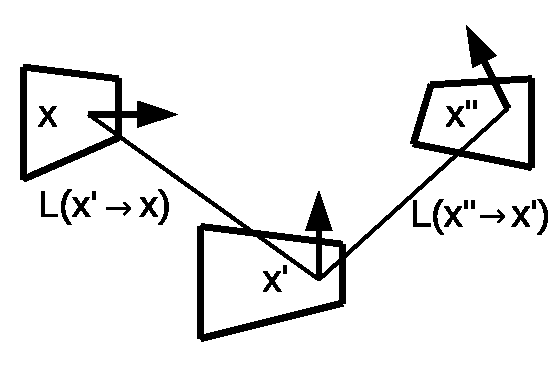
\includegraphics[scale = 0.4]{../figures/rendequation}}
\vspace{-1cm}
$$ L(\bold{x'} \rightarrow \bold{x}) =  g(\bold{x'}  \rightarrow \bold{x})  \left[ \epsilon(\bold{x'}  \rightarrow \bold{x}) + \int_{s}{\rho(\bold{x''}  \rightarrow \bold{x'}  \rightarrow \bold{x})L(\bold{x''}  \rightarrow \bold{x}) d\bold{x''}} \right] $$

\textbf{Recursiva}

$\bold{x}$,$\bold{x'}$ y $\bold{x''}$ varían sobre todas las superficies.

(Ray Tracing, Path Tracing)

\end{frame}

\begin{frame}{Ecuación del Renderizado de Volúmenes}
Cambio de radiancia ($L$) en una dirección dada ($\vec{\omega}$) 

Absorción, dispersión saliente, emisión y dispersión entrante.
\begin{equation*}
\begin{aligned}
(\vec{\omega} \cdot \nabla) L(\bold{x} \rightarrow \vec{\omega}) = - \sigma_{a}(\bold{x}) L(\bold{x} \rightarrow \vec{\omega}) - \sigma_{s}(\bold{x}) L(\bold{x} \rightarrow \vec{\omega}) + \\
\sigma_{a}(\bold{x}) L_{e}(\bold{x} \rightarrow \vec{\omega}) + \sigma_{s}(\bold{x}) L_{i}(\bold{x} \rightarrow \vec{\omega}).
\end{aligned}
\end{equation*}

$\sigma_{a}$: coef. absorción, $\sigma_{s}$: coef. dispersión.

\centering
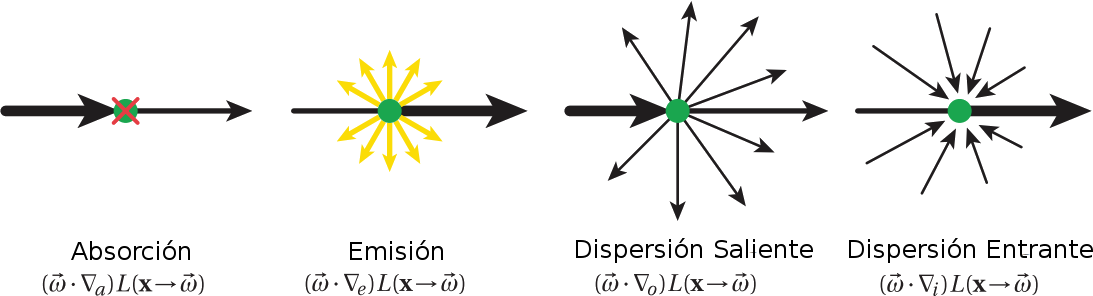
\includegraphics[scale = 0.3]{../figures/fenomenosrte}

Ray Casting (Direct Volume Rendering)
\end{frame}



\begin{frame}{Renderización}

Se propone \textbf{textura volumétrica} $\rightarrow$ \textbf{Renderizado Directo de Volúmenes} (DVR)

\begin{itemize}
\item Evita construcción de una malla.
\item Permite \textbf{cortes arbitrarios} del material (trivialmente).
\end{itemize}

Se computa un \textbf{rayo} para cada pixel, desde la pantalla al objeto.

\textbf{Cambio de radiancia} del rayo a lo largo del medio.


\centerline{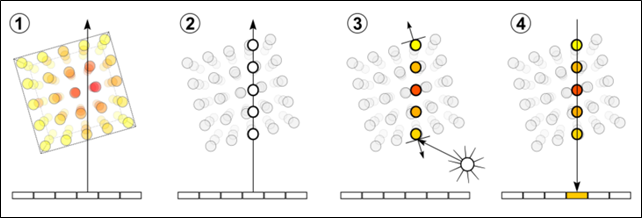
\includegraphics[width=7cm]{../figures/dvr}}

Para obtener resultados en tiempo real, tomamos una versión simplificada de la RTE, teniendo en cuenta solamente la \textbf{transmitancia}.
\end{frame}
\begin{frame}{DVR en GPU}

\begin{itemize}
\item Computamos un \textbf{rayo principal} desde la cámara hacia el volumen
\item \textbf{Sombras}: cada paso del rayo origina un \textbf{rayo secundario}, computando la transmitancia desde la posición actual hacia la luz
\end{itemize}

\centerline{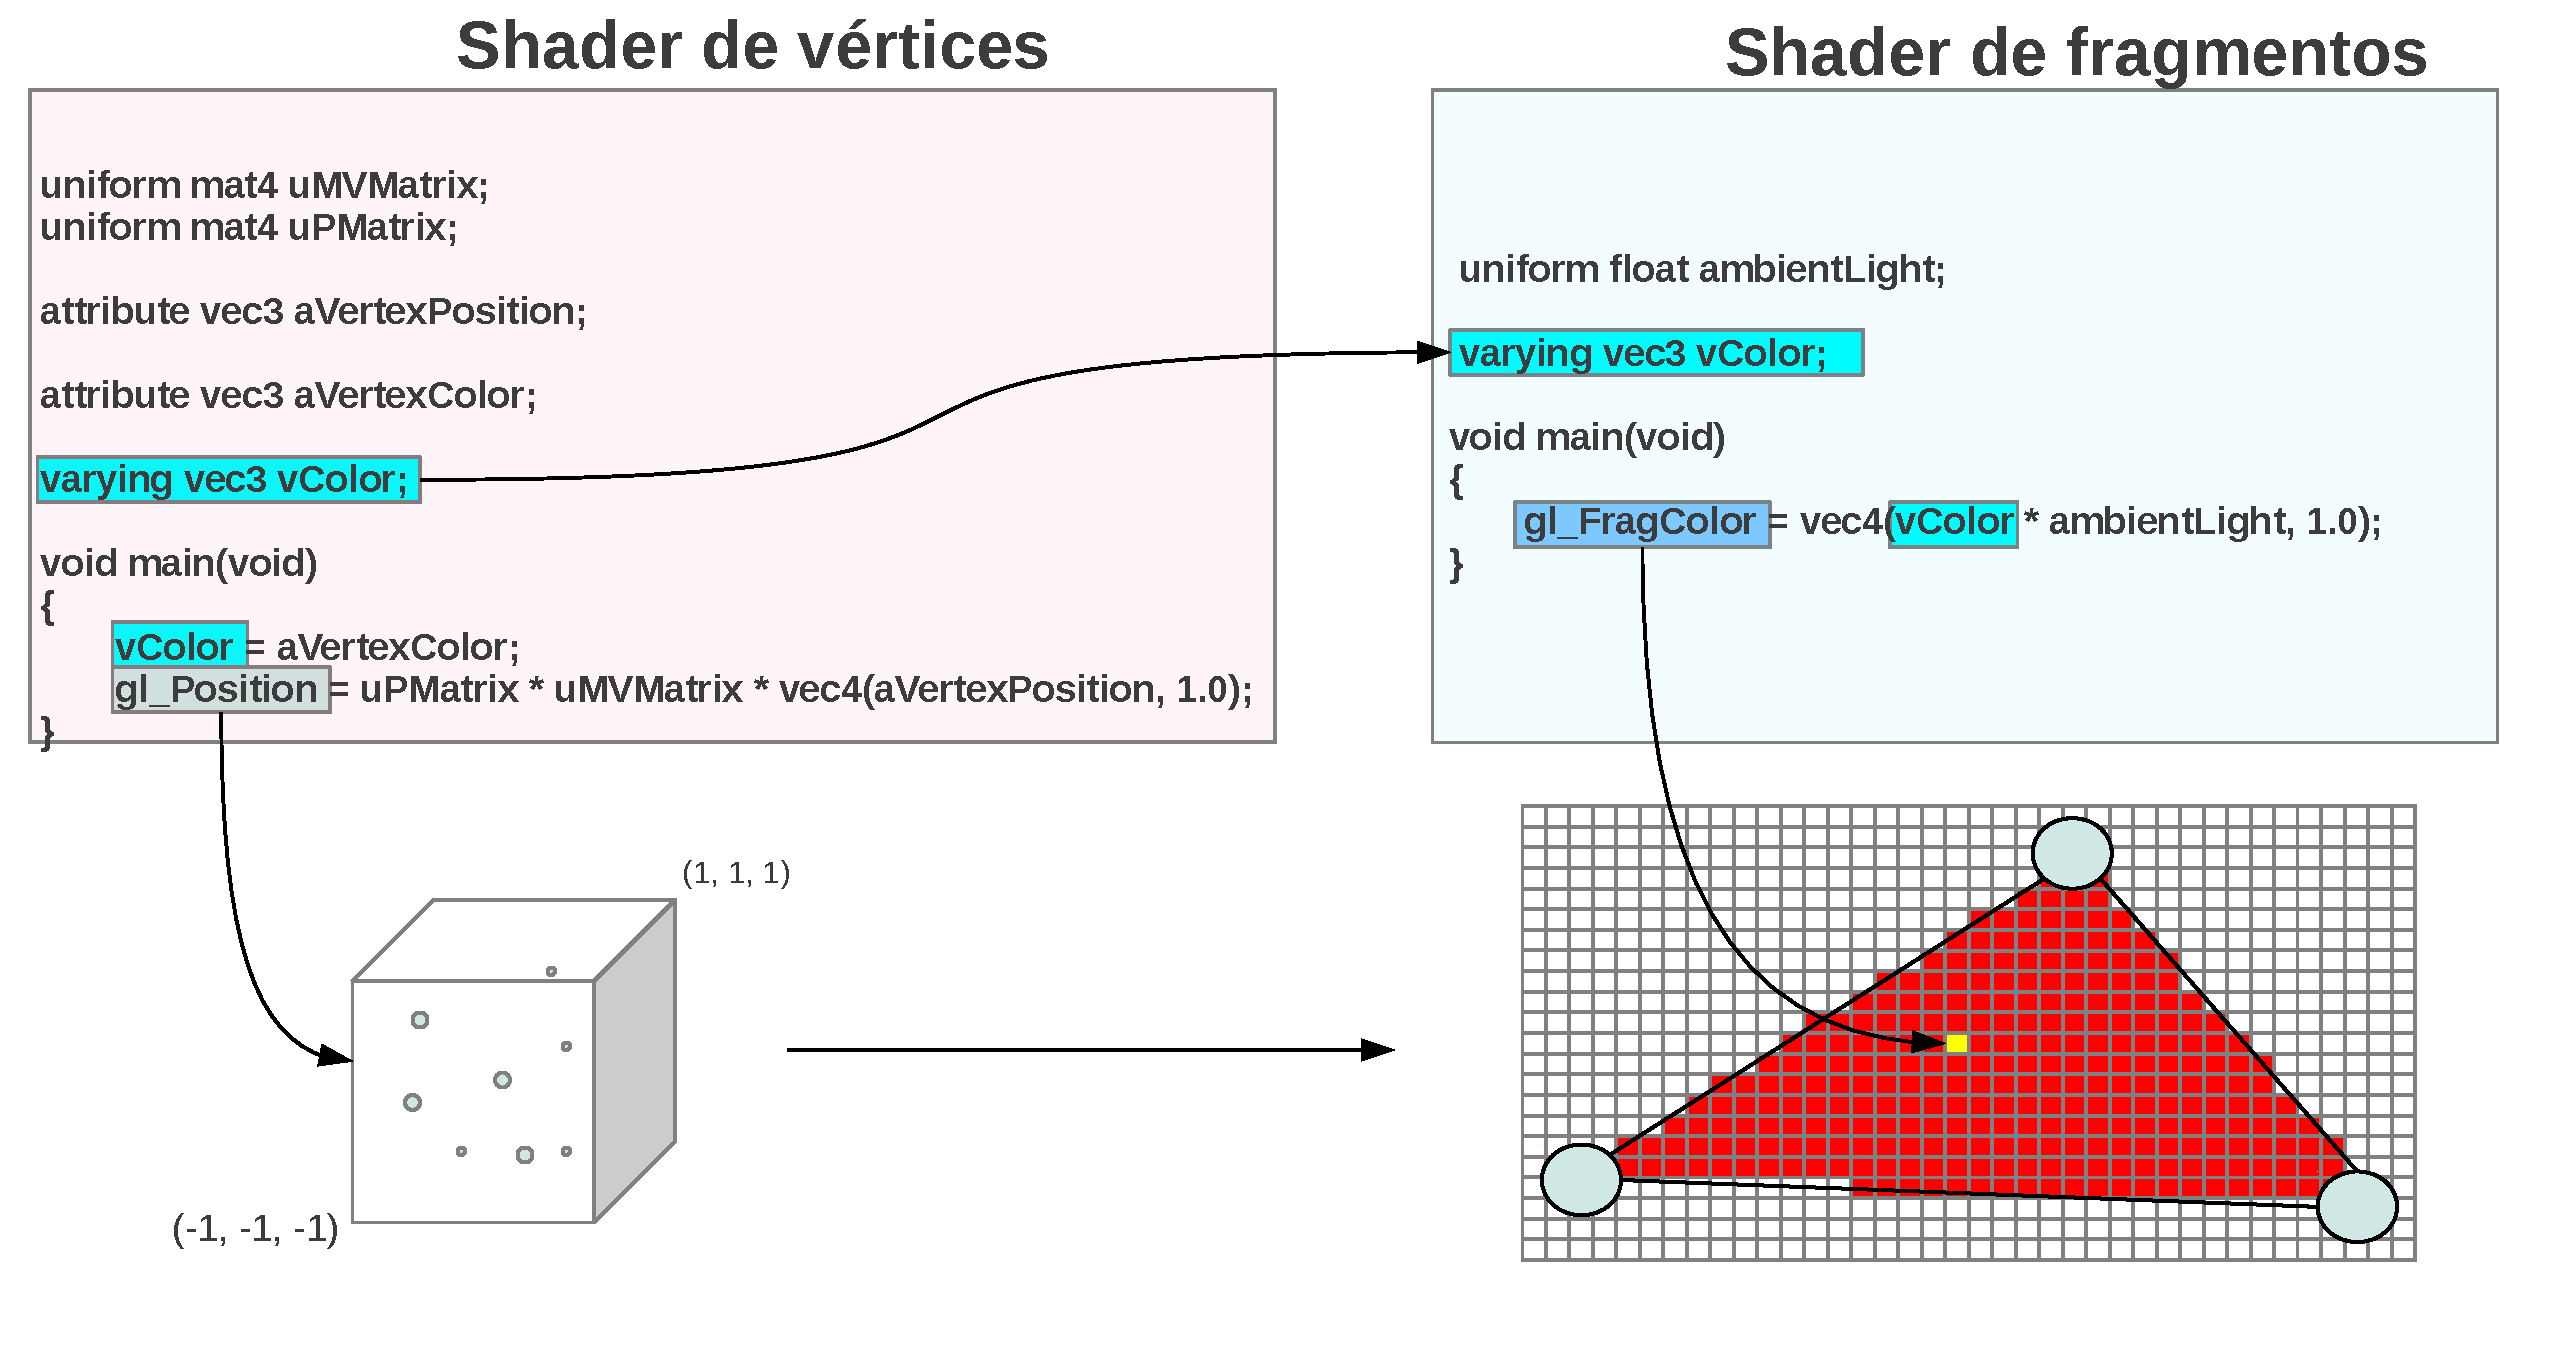
\includegraphics[width=4cm]{../figures/fragmentshader}}

\end{frame}

\begin{frame}
Implementación en GPU, (\textbf{fragment shader}, dentro del \textbf{pipeline gráfico}).

\centerline{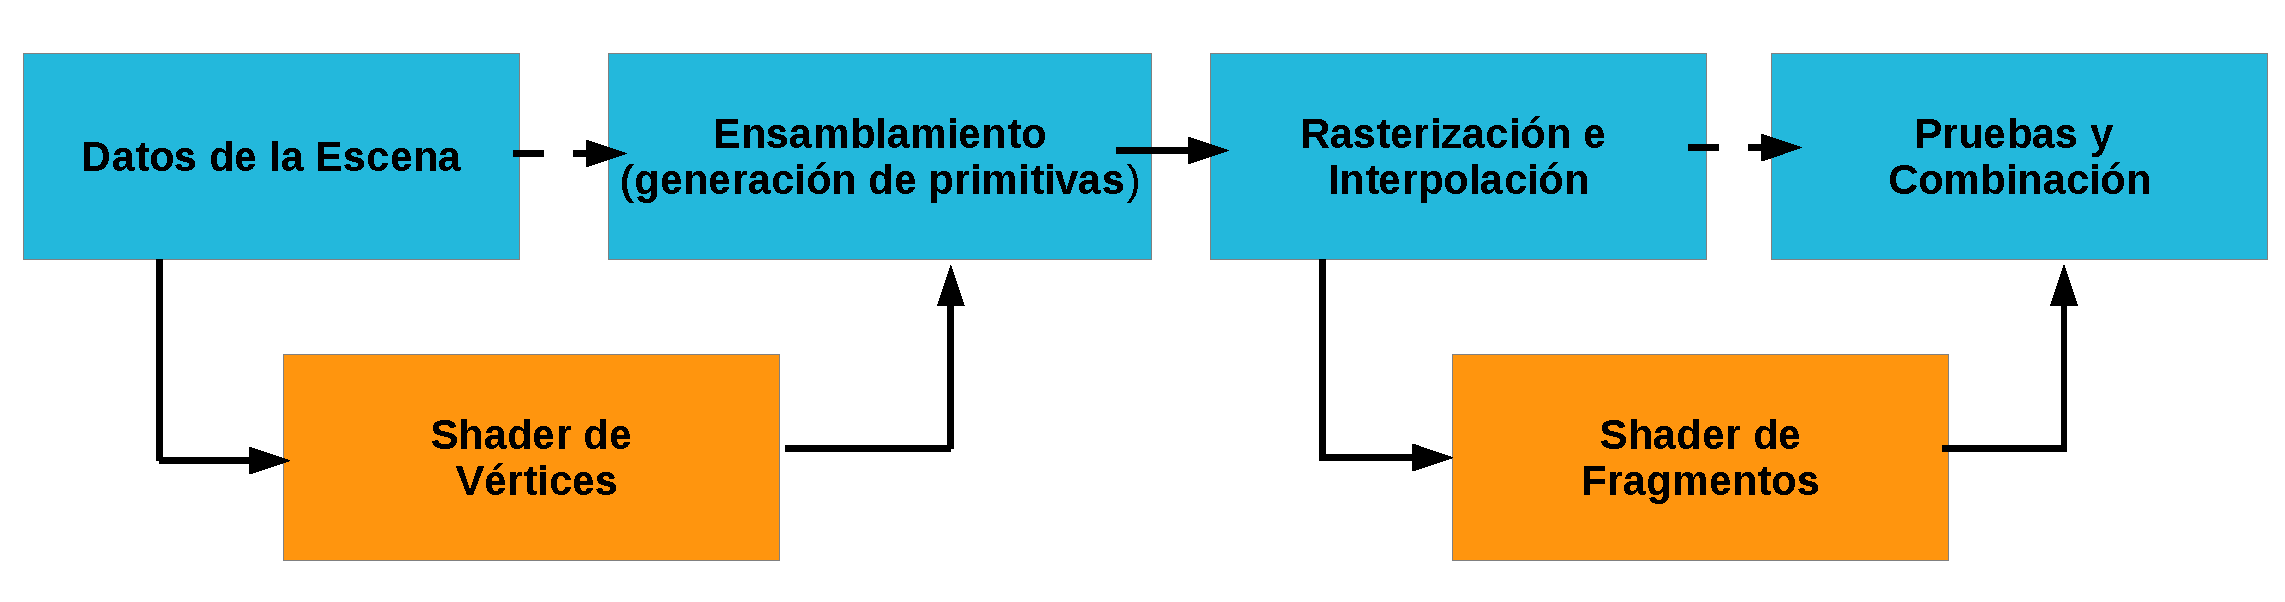
\includegraphics[width=13cm]{../figures/pipelinegrafico}}

\begin{table}[htb]
\centering

\begin{tabular}{|c|c|c|c|c|c|c|}
\hline
 Pasos del rayo         & 128 &  256 \\
\hline
\hline
 Tiempo total shaders   & 10 ms &  32.5 ms \\
\hline
 Rayo Principal         & 2 ms  & 5 ms  \\
\hline
 Rayos Secundarios      &  8 ms & 27.5 ms  \\
\hline
\end{tabular}
\caption{Detalle de tiempos de renderizado en milisegundos.}
\label{tab:n2}
\end{table}


\end{frame}


\begin{frame}{Conclusiones\footnote{Modelado para la Renderización foto-realista de pan, {\it Mecánica Computacional}, Baravalle et.al. 2014}}
\begin{itemize}
\item Imágenes realistas
\item Tiempo interactivo/real
\item Implementación simple en GPU
\end{itemize}

\begin{block}{Trabajos a Futuro}
\begin{itemize}
\item Otros materiales
\item Pre-cómputo de la radiancia
\end{itemize}
\end{block}
\end{frame}

\subsection{Extra}

\begin{frame}
\begin{block}{}
\begin{center}
\vspace{1cm}
\huge{Extra}
\vspace{1cm}
\end{center}
\end{block}
\end{frame}

\begin{frame}{Clasificación de Imágenes de cortes de Pan}
Se estudió el espectro multifractal para \textbf{caracterizar y clasificar} imágenes de cortes reales de pan (baguette, sandwich, lactal, etc.) (Parámetros de calidad que deben respetar los panes reales, clasificación automática)\footnote{Multifractal Characterisation and Classification of Bread Crumb Digital Images, {\it EURASIP Journal on Image and Video Processing}, Baravalle et.al. 2015}

\begin{table}[h!]
\center
\begin{tabular}{lllllll}
\hline\noalign{\smallskip}
Método & Haralick & Lbp & SIFT & MFS & MFS CIELab\\
\noalign{\smallskip}\hline\noalign{\smallskip}
SVM & 94\% & 78.5\% & 96.5\% & 94.5\% & \textbf{97.5\%} \\
RF  & 91\% & 71.5\% & 92\% & 93.5\% & \textbf{96\%} \\
NN & 79\% & 70\% & 86\%  & 90.5\% & \textbf{92\%} \\
\noalign{\smallskip}\hline
\#FDs & 13 & 36 & 128 & 20 & 60\\
\hline
\end{tabular}
\label{tab:other} 
\end{table}

Se encontraron correlaciones entre las dimensiones del MFS, la fracción de vacío (VF) y el área media de las burbujas


\end{frame}

\section[Conclusiones]{Conclusiones y Trabajos a Futuro}


\begin{frame}
\begin{block}{}
\begin{center}
\vspace{1cm}
\huge{Conclusiones y Trabajos a Futuro}
\vspace{1cm}
\end{center}
\end{block}
\end{frame}

\subsection{Conclusiones}
\begin{frame}{Conclusiones}
\begin{block}{}
\begin{itemize}
\item Se introdujo un \textbf{algoritmo procedimental} de generación de geometrías \textbf{porosas} creíbles de manera automática.
\item Se presentó un algoritmo \textbf{basado} en el \textbf{proceso real de formación del pan}, eliminando decisiones ad-hoc en la generación de este material, obteniendo estructuras a lo largo de todo el \textbf{proceso de formación}.
\item Se aplicó un algoritmo de renderizado, basado en la interacción lumínica con una escena, produciendo imágenes foto-realísticas de materiales porosos/cocidos/comestibles como pan, esponjas, y piedras. Se obtuvieron imágenes \textbf{foto-realísticas en tiempo real}, por medio de la utilización de la \textbf{GPU}.
\item Se \textbf{validaron} las geometrías generadas por el proceso inspirado en la formación del pan con muestras reales de pan.
\item Se presentó un método para \textbf{clasificar} muestras de pan, superando a clasificadores del estado del arte.
\end{itemize}
\end{block}
\end{frame}

\subsection{Trabajos a Futuro}
\begin{frame}{Trabajos a Futuro}
\begin{block}{}
\begin{itemize}
\item Generación procedimental de huesos y \textbf{otros materiales}
\item Validación tridimensional de los resultados
\item Implementación en \textbf{GPU} de la \textbf{generación procedimental}
\item Producir un {\it plug-in} de blender (o similar)
\item Validación utilizando técnicas de aprendizaje profundo
\end{itemize}
\end{block}
\end{frame}


\begin{frame}{Validación utilizando Técnicas de Aprendizaje Profundo?}


\centering
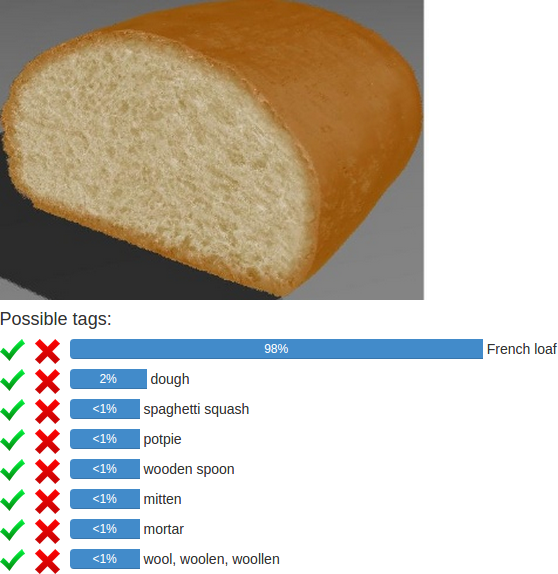
\includegraphics[width=3cm]{../figures/deep1}
\includegraphics[width=3cm]{../figures/deep4}

\includegraphics[width=3cm]{../figures/deep2}
\includegraphics[width=3cm]{../figures/deep3}


\vspace{0.4cm}
\url{http://deeplearning.cs.toronto.edu/}

\end{frame}


\begin{frame}
\centering

?`Preguntas?

\end{frame}

\begin{frame}
\centering

!`Gracias!

\end{frame}
\end{document}
